% Options for packages loaded elsewhere
\PassOptionsToPackage{unicode}{hyperref}
\PassOptionsToPackage{hyphens}{url}
%
\documentclass[
]{article}
\usepackage{amsmath,amssymb}
\usepackage{iftex}
\ifPDFTeX
  \usepackage[T1]{fontenc}
  \usepackage[utf8]{inputenc}
  \usepackage{textcomp} % provide euro and other symbols
\else % if luatex or xetex
  \usepackage{unicode-math} % this also loads fontspec
  \defaultfontfeatures{Scale=MatchLowercase}
  \defaultfontfeatures[\rmfamily]{Ligatures=TeX,Scale=1}
\fi
\usepackage{lmodern}
\ifPDFTeX\else
  % xetex/luatex font selection
\fi
% Use upquote if available, for straight quotes in verbatim environments
\IfFileExists{upquote.sty}{\usepackage{upquote}}{}
\IfFileExists{microtype.sty}{% use microtype if available
  \usepackage[]{microtype}
  \UseMicrotypeSet[protrusion]{basicmath} % disable protrusion for tt fonts
}{}
\makeatletter
\@ifundefined{KOMAClassName}{% if non-KOMA class
  \IfFileExists{parskip.sty}{%
    \usepackage{parskip}
  }{% else
    \setlength{\parindent}{0pt}
    \setlength{\parskip}{6pt plus 2pt minus 1pt}}
}{% if KOMA class
  \KOMAoptions{parskip=half}}
\makeatother
\usepackage{xcolor}
\usepackage[margin=1in]{geometry}
\usepackage{color}
\usepackage{fancyvrb}
\newcommand{\VerbBar}{|}
\newcommand{\VERB}{\Verb[commandchars=\\\{\}]}
\DefineVerbatimEnvironment{Highlighting}{Verbatim}{commandchars=\\\{\}}
% Add ',fontsize=\small' for more characters per line
\usepackage{framed}
\definecolor{shadecolor}{RGB}{248,248,248}
\newenvironment{Shaded}{\begin{snugshade}}{\end{snugshade}}
\newcommand{\AlertTok}[1]{\textcolor[rgb]{0.94,0.16,0.16}{#1}}
\newcommand{\AnnotationTok}[1]{\textcolor[rgb]{0.56,0.35,0.01}{\textbf{\textit{#1}}}}
\newcommand{\AttributeTok}[1]{\textcolor[rgb]{0.13,0.29,0.53}{#1}}
\newcommand{\BaseNTok}[1]{\textcolor[rgb]{0.00,0.00,0.81}{#1}}
\newcommand{\BuiltInTok}[1]{#1}
\newcommand{\CharTok}[1]{\textcolor[rgb]{0.31,0.60,0.02}{#1}}
\newcommand{\CommentTok}[1]{\textcolor[rgb]{0.56,0.35,0.01}{\textit{#1}}}
\newcommand{\CommentVarTok}[1]{\textcolor[rgb]{0.56,0.35,0.01}{\textbf{\textit{#1}}}}
\newcommand{\ConstantTok}[1]{\textcolor[rgb]{0.56,0.35,0.01}{#1}}
\newcommand{\ControlFlowTok}[1]{\textcolor[rgb]{0.13,0.29,0.53}{\textbf{#1}}}
\newcommand{\DataTypeTok}[1]{\textcolor[rgb]{0.13,0.29,0.53}{#1}}
\newcommand{\DecValTok}[1]{\textcolor[rgb]{0.00,0.00,0.81}{#1}}
\newcommand{\DocumentationTok}[1]{\textcolor[rgb]{0.56,0.35,0.01}{\textbf{\textit{#1}}}}
\newcommand{\ErrorTok}[1]{\textcolor[rgb]{0.64,0.00,0.00}{\textbf{#1}}}
\newcommand{\ExtensionTok}[1]{#1}
\newcommand{\FloatTok}[1]{\textcolor[rgb]{0.00,0.00,0.81}{#1}}
\newcommand{\FunctionTok}[1]{\textcolor[rgb]{0.13,0.29,0.53}{\textbf{#1}}}
\newcommand{\ImportTok}[1]{#1}
\newcommand{\InformationTok}[1]{\textcolor[rgb]{0.56,0.35,0.01}{\textbf{\textit{#1}}}}
\newcommand{\KeywordTok}[1]{\textcolor[rgb]{0.13,0.29,0.53}{\textbf{#1}}}
\newcommand{\NormalTok}[1]{#1}
\newcommand{\OperatorTok}[1]{\textcolor[rgb]{0.81,0.36,0.00}{\textbf{#1}}}
\newcommand{\OtherTok}[1]{\textcolor[rgb]{0.56,0.35,0.01}{#1}}
\newcommand{\PreprocessorTok}[1]{\textcolor[rgb]{0.56,0.35,0.01}{\textit{#1}}}
\newcommand{\RegionMarkerTok}[1]{#1}
\newcommand{\SpecialCharTok}[1]{\textcolor[rgb]{0.81,0.36,0.00}{\textbf{#1}}}
\newcommand{\SpecialStringTok}[1]{\textcolor[rgb]{0.31,0.60,0.02}{#1}}
\newcommand{\StringTok}[1]{\textcolor[rgb]{0.31,0.60,0.02}{#1}}
\newcommand{\VariableTok}[1]{\textcolor[rgb]{0.00,0.00,0.00}{#1}}
\newcommand{\VerbatimStringTok}[1]{\textcolor[rgb]{0.31,0.60,0.02}{#1}}
\newcommand{\WarningTok}[1]{\textcolor[rgb]{0.56,0.35,0.01}{\textbf{\textit{#1}}}}
\usepackage{graphicx}
\makeatletter
\def\maxwidth{\ifdim\Gin@nat@width>\linewidth\linewidth\else\Gin@nat@width\fi}
\def\maxheight{\ifdim\Gin@nat@height>\textheight\textheight\else\Gin@nat@height\fi}
\makeatother
% Scale images if necessary, so that they will not overflow the page
% margins by default, and it is still possible to overwrite the defaults
% using explicit options in \includegraphics[width, height, ...]{}
\setkeys{Gin}{width=\maxwidth,height=\maxheight,keepaspectratio}
% Set default figure placement to htbp
\makeatletter
\def\fps@figure{htbp}
\makeatother
\setlength{\emergencystretch}{3em} % prevent overfull lines
\providecommand{\tightlist}{%
  \setlength{\itemsep}{0pt}\setlength{\parskip}{0pt}}
\setcounter{secnumdepth}{-\maxdimen} % remove section numbering
\ifLuaTeX
  \usepackage{selnolig}  % disable illegal ligatures
\fi
\IfFileExists{bookmark.sty}{\usepackage{bookmark}}{\usepackage{hyperref}}
\IfFileExists{xurl.sty}{\usepackage{xurl}}{} % add URL line breaks if available
\urlstyle{same}
\hypersetup{
  pdftitle={Práctica 2},
  pdfauthor={Autor: Christian Rolando Oyola Flores},
  hidelinks,
  pdfcreator={LaTeX via pandoc}}

\title{Práctica 2}
\author{Autor: Christian Rolando Oyola Flores}
\date{Tipología y ciclo de vida de los datos - Semestre 2023}

\begin{document}
\maketitle

{
\setcounter{tocdepth}{2}
\tableofcontents
}
\begin{center}\rule{0.5\linewidth}{0.5pt}\end{center}

\hypertarget{introducciuxf3n}{%
\section{1 Introducción}\label{introducciuxf3n}}

\begin{center}\rule{0.5\linewidth}{0.5pt}\end{center}

\hypertarget{presentaciuxf3n}{%
\subsection{1.1 Presentación}\label{presentaciuxf3n}}

En esta práctica se elabora un caso práctico orientado a aprender a
identificar los datos relevantes para un proyecto analítico y usar las
herramientas de integración, limpieza, validación y análisis de los
mismos

\hypertarget{objetivos}{%
\subsection{1.2 Objetivos}\label{objetivos}}

Los objetivos concretos de esta práctica son:

\begin{itemize}
\tightlist
\item
  Aprender a aplicar los conocimientos adquiridos y su capacidad de
  resolución de problemas en entornos nuevos o poco conocidos dentro de
  contextos más amplios o multidisciplinares.
\item
  Saber identificar los datos relevantes y los tratamientos necesarios
  (integración, limpieza y validación) para llevar a cabo un proyecto
  analítico.
\item
  Aprender a analizar los datos adecuadamente para abordar la
  información contenida en los datos.
\item
  Identificar la mejor representación de los resultados para aportar
  conclusiones sobre el problema planteado en el proceso analítico.
\item
  Actuar con los principios éticos y legales relacionados con la
  manipulación de datos en función del ámbito de aplicación.
\item
  Desarrollar las habilidades de aprendizaje que les permitan continuar
  estudiando de un modo que tendrá que ser en gran medida autodirigido o
  autónomo.
\item
  Desarrollar la capacidad de búsqueda, gestión y uso de información y
  recursos en el ámbito de la ciencia de datos
\end{itemize}

\hypertarget{competencias}{%
\subsection{1.3 Competencias}\label{competencias}}

En esta práctica se desarrollan las siguientes competencias del Máster
de Data Science:

\begin{itemize}
\tightlist
\item
  Capacidad de analizar un problema en el nivel de abstracción adecuado
  a cada situación y aplicar las habilidades y conocimientos adquiridos
  para abordarlo y resolverlo.
\item
  Capacidad para aplicar las técnicas específicas de tratamiento de
  datos (integración, transformación, limpieza y validación) para su
  posterior análisis.
\end{itemize}

\begin{center}\rule{0.5\linewidth}{0.5pt}\end{center}

\hypertarget{planteamiento-de-objetivos-analuxedticos-y-descripciuxf3n-detallada-de-la-metodologuxeda-para-su-resoluciuxf3n}{%
\section{2 Planteamiento de objetivos analíticos y descripción detallada
de la metodología para su
resolución}\label{planteamiento-de-objetivos-analuxedticos-y-descripciuxf3n-detallada-de-la-metodologuxeda-para-su-resoluciuxf3n}}

\begin{center}\rule{0.5\linewidth}{0.5pt}\end{center}

El propósito fundamental de este desarrollo es examinar e identificar
las variables de riesgo asociadas con problemas cardíacos en una
población específica. La identificación de estos factores es crucial
para desarrollar modelos predictivos que puedan contribuir en la
detección temprana y en la generación de alertas sobre problemas
cardíacos. En este contexto, se plantea suministrar información crucial
a las instituciones de salud pública sobre los factores relacionados con
problemas cardíacos. Esta información está destinada a facilitar la
creación de políticas o programas preventivos en el ámbito de la salud,
enfocados en mitigar y manejar eficazmente esta problemática.

En este contexto, el análisis estadístico se centrará en el examen de
datos históricos de pacientes que hayan experimentado cuadros clínicos
asociados a problemas cardíacos. Esto permitirá identificar perfiles de
riesgo basándose en varias dimensiones de interés: demográficas,
análisis clínicos y clasificación de riesgos. Cada una de estas
dimensiones aportará información vital para comprender mejor los
factores que contribuyen a estos problemas de salud y facilitar así la
toma de decisiones informadas.

La metodología para abordar el objetivo planteado incluye los siguientes
procesos:

\begin{enumerate}
\def\labelenumi{\alph{enumi}.}
\tightlist
\item
  Análisis exploratorio de datos:
\end{enumerate}

\begin{itemize}
\tightlist
\item
  Se llevará a cabo un análisis inicial de las variables definidas en el
  conjunto de datos, incluyendo su tipo (categórica, numérica, binaria),
  y su distribución.
\item
  Identificar y tratar los valores faltantes o datos atípicos que puedan
  afectar al estudio.
\item
  En esta misma línea, se llevará a cabo un proceso de identificación de
  las relaciones entre las variables, apoyados sobre gráficos y técnicas
  estadísticas para obtener una comprensión optima del conjunto de
  datos.
\end{itemize}

\begin{enumerate}
\def\labelenumi{\alph{enumi}.}
\setcounter{enumi}{1}
\tightlist
\item
  Preprocesamiento de datos:
\end{enumerate}

\begin{itemize}
\tightlist
\item
  Dentro de esta etapa se llevará a cabo una codificación (según
  corresponda) de las variables categóricas.
\item
  Así también, es relevante para el caso de estudio escalar o
  estandarizar las variables numéricas, esto con el objetivo de asegurar
  que todas las variables tengan un rango comparable.
\end{itemize}

\hypertarget{selecciuxf3n-del-juego-de-datos}{%
\subsection{2.1 Selección del juego de
datos}\label{selecciuxf3n-del-juego-de-datos}}

\hypertarget{justificaciuxf3n-de-elecciuxf3n-del-set-de-datos}{%
\subsubsection{2.1.1 Justificación de elección del set de
datos}\label{justificaciuxf3n-de-elecciuxf3n-del-set-de-datos}}

La elección del conjunto de datos
\href{https://www.kaggle.com/datasets/rashikrahmanpritom/heart-attack-analysis-prediction-dataset}{Heart
Attack Analysis \& Prediction Dataset} del repositorio kaggle, se basa
en su idoneidad para aplicar una variedad de técnicas de análisis y
exploración de informacíón para llevar a cabo un proyecto analítico,

Este único conjunto de datos contiene información sobre factores
vinculados con ataques cardiacos en una población, vinculando
adicionalmente variables numéricas y categóricas, así momo, la
vinculación de variables de salida para la predicción de pacientes que
puede presentar esta problemática.

Con una variable objetivo (target) claramente definida y un conjunto
diverso de variables predictoras relacionadas con los pacientes, este
conjunto de datos se presta para un análisis más exhaustivo. Este
análisis podría incluir la aplicación de algoritmos supervisados de
clasificación y regresión, orientados a predecir y entender los factores
que inciden en los ataques cardíacos.

\hypertarget{descripciuxf3n-del-dataset}{%
\subsubsection{2.1.2 Descripción del
dataset}\label{descripciuxf3n-del-dataset}}

La selección de este dataset permitirá llevar a cabo un análisis de
factores que contribuyen a los ataques cardíacos, este conjunto de datos
puede ayudar a desarrollar modelos predictivos, partiendo de una
identificación inicial de input's o variables vinculadas. Estos modelos
podrían ser utilizados por los profesionales de la salud para
identificar a los individuos con alto riesgo de sufrir un ataque
cardíaco, permitiendo llevar a cabo intervenciones preventivas y
diagnósticos tempranos. Las preguntas o problemas específicos que se
pretende responder o abordar con este conjunto de datos incluyen:

\begin{itemize}
\tightlist
\item
  ¿Cuales son lor principales factores predictivos de un ataque
  cardiaco?
\item
  ¿Cómo afectan el ejercicio y la dieta al riesgo de ataques cardíacos?
\item
  ¿Cómo difieren los síntomas y factores de riesgo entre hombres y
  mujeres?
\item
  ¿Cómo cambia el riesgo y la presentación de enfermedades cardíacas con
  la edad?
\end{itemize}

\hypertarget{integraciuxf3n-y-selecciuxf3n-de-los-datos-de-interes}{%
\subsubsection{2.1.3 Integración y selección de los datos de
interes}\label{integraciuxf3n-y-selecciuxf3n-de-los-datos-de-interes}}

Para el desarrollo de esta práctica, se integrarán las 14 variables
presentes en el conjunto de datos original, utilizando así todas las
características disponibles. Para facilitar este proceso, crearemos un
diccionario de datos basándonos en la documentación auxiliar
proporcionada. Este diccionario será una herramienta clave para mejorar
la comprensión de la importancia y el significado de cada variable en el
contexto del estudio constituido en 3 dimensiones de análisis:

\textbf{Dimensión Demográfica:}

\begin{itemize}
\tightlist
\item
  \textbf{age} - edad en años
\item
  \textbf{sex} - sexo (1 = masculino; 0 = femenino)
\end{itemize}

\textbf{Dimensión Análisis Clinico:}

\begin{itemize}
\tightlist
\item
  \textbf{cp} - tipo de dolor torácico (1 = angina típica; 2 = angina
  atípica; 3 = dolor no anginoso; 0 = asintomático)
\item
  \textbf{trestbps} - presión arterial en reposo (en mm Hg al ingreso al
  hospital)
\item
  \textbf{chol} - colesterol sérico en mg/dl
\item
  \textbf{fbs} - glucosa en sangre en ayunas \textgreater{} 120 mg/dl (1
  = cierto; 0 = falso)
\item
  \textbf{restecg} - resultados electrocardiográficos en reposo (1 =
  normal; 2 = anormalidad de onda ST-T; 0 = hipertrofia)
\item
  \textbf{thalachh} - máxima frecuencia cardíaca alcanzada
\item
  \textbf{exng} - angina inducida por ejercicio (1 = sí; 0 = no)
\item
  \textbf{oldpeak} - depresión del segmento ST inducida por ejercicio
  relativo al reposo
\item
  \textbf{slp} - la pendiente del segmento ST del ejercicio máximo (2 =
  ascendente; 1 = plano; 0 = descendente)
\item
  \textbf{caa} - número de vasos principales (0-3) coloreados por
  fluoroscopia
\item
  \textbf{thall} - 2 = normal; 1 = defecto fijo; 3 = defecto reversible
\end{itemize}

\textbf{Dimensión Clasificación:}

\begin{itemize}
\tightlist
\item
  \textbf{output: 0} = menor probabilidad de ataque al corazón 1 = mayor
  probabilidad de ataque al corazón
\end{itemize}

Después de definir el diccionario y especificar los tipos de datos,
procederemos a realizar un análisis más detallado de los datos que
conforman dicho diccionario.

\begin{center}\rule{0.5\linewidth}{0.5pt}\end{center}

\hypertarget{limpieza-de-datos}{%
\subsection{2.2 Limpieza de datos}\label{limpieza-de-datos}}

Para comenzar el análisis, importamos el conjunto de datos en una
estructura de datos adecuada utilizando bibliotecas especializadas en
manipulación y análisis de datos.

\emph{Cargamos los datos de un directorio local:}

\begin{Shaded}
\begin{Highlighting}[]
\NormalTok{heart\_csv }\OtherTok{\textless{}{-}} \FunctionTok{read\_delim}\NormalTok{(}\StringTok{"Data/heart.csv"}\NormalTok{, }\CommentTok{\#lectura del archivo empleando la función read\_delim()}
            \AttributeTok{delim =} \StringTok{","}\NormalTok{, }\CommentTok{\#especificación del delimitador en la lectura del archivo.}
            \AttributeTok{escape\_double =} \ConstantTok{FALSE}\NormalTok{, }\CommentTok{\#no se deben "escapar" las comillas dobles presentes en el archivo.}
            \AttributeTok{trim\_ws =} \ConstantTok{TRUE}\NormalTok{) }\CommentTok{\#se deben eliminar los espacios en blanco de los valores en el archivo}
\end{Highlighting}
\end{Shaded}

\hypertarget{inspecciuxf3n-inicial-de-datos}{%
\subsubsection{2.2.1 Inspección inicial de
datos}\label{inspecciuxf3n-inicial-de-datos}}

Realizamos una inspección inicial de los datos con el fin de obtener una
visión general de la estructura y el formato de los atributos. Durante
esta etapa, verificamos el número de filas y columnas, revisamos los
nombres de las columnas y observamos los primeros registros del
DataFrame. Este proceso nos permite familiarizarnos con los datos y nos
ayuda a considerar lo siguiente:

\begin{itemize}
\tightlist
\item
  \textbf{¿Qué representa cada atributo?}
\item
  \textbf{¿Qué tipo de dato debería tener cada columna?}
\item
  \textbf{¿Que granularidad o atomicidad tiene la data?}
\end{itemize}

\emph{a) Mostramos la estructura del conjunto de datos:}

\begin{Shaded}
\begin{Highlighting}[]
\NormalTok{data\_heart }\OtherTok{\textless{}{-}}\NormalTok{ heart\_csv}
\FunctionTok{glimpse}\NormalTok{(data\_heart) }\CommentTok{\# vista resumida de la estructura del dataset}
\end{Highlighting}
\end{Shaded}

\begin{verbatim}
## Rows: 303
## Columns: 14
## $ age      <dbl> 63, 37, 41, 56, 57, 57, 56, 44, 52, 57, 54, 48, 49, 64, 58, 5~
## $ sex      <dbl> 1, 1, 0, 1, 0, 1, 0, 1, 1, 1, 1, 0, 1, 1, 0, 0, 0, 0, 1, 0, 1~
## $ cp       <dbl> 3, 2, 1, 1, 0, 0, 1, 1, 2, 2, 0, 2, 1, 3, 3, 2, 2, 3, 0, 3, 0~
## $ trtbps   <dbl> 145, 130, 130, 120, 120, 140, 140, 120, 172, 150, 140, 130, 1~
## $ chol     <dbl> 233, 250, 204, 236, 354, 192, 294, 263, 199, 168, 239, 275, 2~
## $ fbs      <dbl> 1, 0, 0, 0, 0, 0, 0, 0, 1, 0, 0, 0, 0, 0, 1, 0, 0, 0, 0, 0, 0~
## $ restecg  <dbl> 0, 1, 0, 1, 1, 1, 0, 1, 1, 1, 1, 1, 1, 0, 0, 1, 1, 1, 1, 1, 1~
## $ thalachh <dbl> 150, 187, 172, 178, 163, 148, 153, 173, 162, 174, 160, 139, 1~
## $ exng     <dbl> 0, 0, 0, 0, 1, 0, 0, 0, 0, 0, 0, 0, 0, 1, 0, 0, 0, 0, 0, 0, 0~
## $ oldpeak  <dbl> 2.3, 3.5, 1.4, 0.8, 0.6, 0.4, 1.3, 0.0, 0.5, 1.6, 1.2, 0.2, 0~
## $ slp      <dbl> 0, 0, 2, 2, 2, 1, 1, 2, 2, 2, 2, 2, 2, 1, 2, 1, 2, 0, 2, 2, 1~
## $ caa      <dbl> 0, 0, 0, 0, 0, 0, 0, 0, 0, 0, 0, 0, 0, 0, 0, 0, 0, 0, 0, 2, 0~
## $ thall    <dbl> 1, 2, 2, 2, 2, 1, 2, 3, 3, 2, 2, 2, 2, 2, 2, 2, 2, 2, 2, 2, 3~
## $ output   <dbl> 1, 1, 1, 1, 1, 1, 1, 1, 1, 1, 1, 1, 1, 1, 1, 1, 1, 1, 1, 1, 1~
\end{verbatim}

Se puede evidenciar que para este dataset se cuenta con un total de
\textbf{303} registros y \textbf{14} variables o caracteristicas. Estos
datos nos proporcionarán la información necesaria para respaldar nuestro
modelo de predicción.

\hypertarget{preprocesamiento-y-gestiuxf3n-de-caracteruxedsticas}{%
\subsection{2.3 Preprocesamiento y gestión de
características}\label{preprocesamiento-y-gestiuxf3n-de-caracteruxedsticas}}

\hypertarget{valores-faltantes}{%
\subsubsection{2.3.1 Valores faltantes}\label{valores-faltantes}}

El siguiente paso será la limpieza de datos, identificando la presencia
de valores vacíos o nulos.

\begin{Shaded}
\begin{Highlighting}[]
\FunctionTok{colSums}\NormalTok{(}\FunctionTok{is.na}\NormalTok{(data\_heart))}
\end{Highlighting}
\end{Shaded}

\begin{verbatim}
##      age      sex       cp   trtbps     chol      fbs  restecg thalachh 
##        0        0        0        0        0        0        0        0 
##     exng  oldpeak      slp      caa    thall   output 
##        0        0        0        0        0        0
\end{verbatim}

\begin{Shaded}
\begin{Highlighting}[]
\FunctionTok{colSums}\NormalTok{(data\_heart}\SpecialCharTok{==}\StringTok{""}\NormalTok{)}
\end{Highlighting}
\end{Shaded}

\begin{verbatim}
##      age      sex       cp   trtbps     chol      fbs  restecg thalachh 
##        0        0        0        0        0        0        0        0 
##     exng  oldpeak      slp      caa    thall   output 
##        0        0        0        0        0        0
\end{verbatim}

En un primer análisis se puede identificar que en el conjunto de datos,
todas las columnas son continuas, no hay columnas completamente vacías,
y todas las filas están completas, es decir, sin observaciones
faltantes.

\hypertarget{valores-outliers}{%
\subsubsection{2.3.2 Valores Outliers}\label{valores-outliers}}

Dentro del proceso de limpieza de datos, se efectúa un análisis de los
valores extremos en las características. El objetivo es identificar y
tratar adecuadamente estos valores para evitar sesgos en el análisis.
Este paso es crucial, ya que los valores extremos pueden distorsionar
los resultados y afectar la precisión de los modelos, para ello usaremos
una representación mediante diagrama de cajas:

\begin{Shaded}
\begin{Highlighting}[]
\CommentTok{\# Ajustar el layout para tener 1 fila y 2 columnas}
\FunctionTok{par}\NormalTok{(}\AttributeTok{mfrow=}\FunctionTok{c}\NormalTok{(}\DecValTok{1}\NormalTok{, }\DecValTok{2}\NormalTok{), }\AttributeTok{las=}\DecValTok{2}\NormalTok{)}
\CommentTok{\# Primer boxplot}
\FunctionTok{boxplot}\NormalTok{(data\_heart[, }\FunctionTok{c}\NormalTok{(}\StringTok{"age"}\NormalTok{, }\StringTok{"cp"}\NormalTok{, }\StringTok{"trtbps"}\NormalTok{, }\StringTok{"chol"}\NormalTok{, }\StringTok{"fbs"}\NormalTok{, }\StringTok{"restecg"}\NormalTok{)], }
        \AttributeTok{main=}\StringTok{"Dimensión Análisis Clínico"}\NormalTok{)}
\CommentTok{\# Segundo boxplot}
\FunctionTok{boxplot}\NormalTok{(data\_heart[, }\FunctionTok{c}\NormalTok{(}\StringTok{"thalachh"}\NormalTok{, }\StringTok{"exng"}\NormalTok{, }\StringTok{"oldpeak"}\NormalTok{, }\StringTok{"slp"}\NormalTok{, }\StringTok{"caa"}\NormalTok{, }\StringTok{"thall"}\NormalTok{)], }
        \AttributeTok{main=}\StringTok{"Dimensión Análisis Clínico"}\NormalTok{)}
\end{Highlighting}
\end{Shaded}

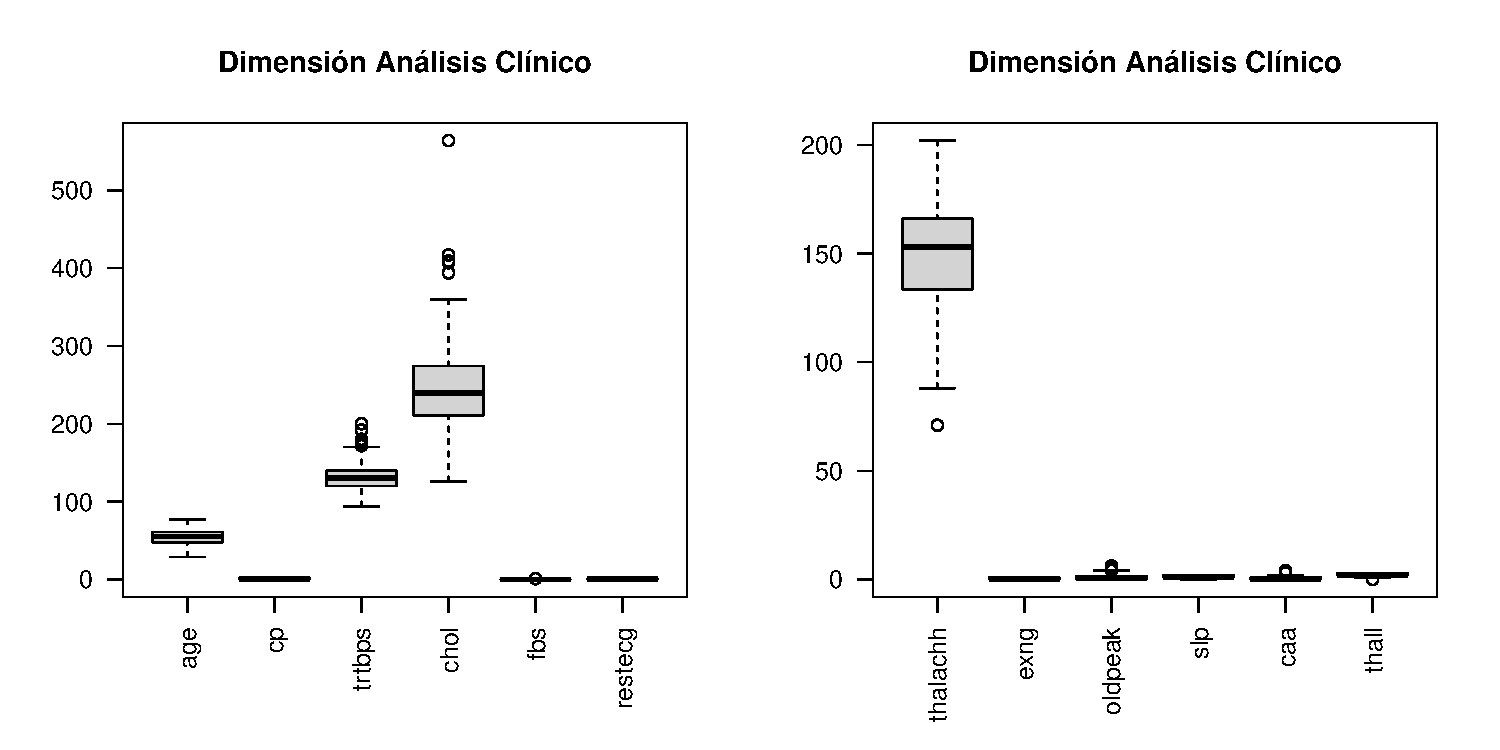
\includegraphics{coyolaf_ChristianOyola-PRA2_files/figure-latex/unnamed-chunk-5-1.pdf}

La observación gráfica inicial permite evidenciar la presencia de
valores extremos en las variables trtbps, chol, thalachh y oldpeak. Para
complementar y confirmar estos hallazgos, es esencial acceder a los
detalles estadísticos referentes a los boxplots, que incluyen los
cuartiles, la mediana y los valores extremos específicos.

\begin{Shaded}
\begin{Highlighting}[]
\NormalTok{chol\_outliers }\OtherTok{\textless{}{-}} \FunctionTok{boxplot.stats}\NormalTok{(data\_heart}\SpecialCharTok{$}\NormalTok{chol)}\SpecialCharTok{$}\NormalTok{out }\CommentTok{\# valores atípicos para \textquotesingle{}chol\textquotesingle{}}
\NormalTok{trtbps\_outliers }\OtherTok{\textless{}{-}} \FunctionTok{boxplot.stats}\NormalTok{(data\_heart}\SpecialCharTok{$}\NormalTok{trtbps)}\SpecialCharTok{$}\NormalTok{out }\CommentTok{\#valores atípicos para \textquotesingle{}trtbps\textquotesingle{}}
\NormalTok{thalachh\_outliers }\OtherTok{\textless{}{-}} \FunctionTok{boxplot.stats}\NormalTok{(data\_heart}\SpecialCharTok{$}\NormalTok{thalachh)}\SpecialCharTok{$}\NormalTok{out }\CommentTok{\#valores atípicos para \textquotesingle{}thalachh\textquotesingle{}}
\NormalTok{oldpeak\_outliers }\OtherTok{\textless{}{-}} \FunctionTok{boxplot.stats}\NormalTok{(data\_heart}\SpecialCharTok{$}\NormalTok{oldpeak)}\SpecialCharTok{$}\NormalTok{out}
\NormalTok{caa\_outliers }\OtherTok{\textless{}{-}} \FunctionTok{boxplot.stats}\NormalTok{(data\_heart}\SpecialCharTok{$}\NormalTok{caa)}\SpecialCharTok{$}\NormalTok{out}
\NormalTok{outliers\_list }\OtherTok{\textless{}{-}} \FunctionTok{list}\NormalTok{(}
  \AttributeTok{Cholesterol\_Outliers =}\NormalTok{ chol\_outliers,}
  \AttributeTok{Resting\_BP\_Outliers =}\NormalTok{ trtbps\_outliers,}
  \AttributeTok{Max\_HR\_Outliers =}\NormalTok{ thalachh\_outliers,}
  \AttributeTok{oldpeak =}\NormalTok{ oldpeak\_outliers,}
  \AttributeTok{Max\_HR\_Outliers =}\NormalTok{ caa\_outliers}
\NormalTok{)}
\end{Highlighting}
\end{Shaded}

Se analiza la influencia de los outliers en relación con la edad de los
pacientes para tomar un criterio más acertado de eliminación o no de los
valores extremos.

\begin{Shaded}
\begin{Highlighting}[]
\CommentTok{\# Crear el primer boxplot para \textquotesingle{}trtbps\textquotesingle{} en función de \textquotesingle{}age\textquotesingle{}}
\NormalTok{bp1 }\OtherTok{\textless{}{-}} \FunctionTok{ggplot}\NormalTok{(}\AttributeTok{data =}\NormalTok{ data\_heart, }\FunctionTok{aes}\NormalTok{(}\AttributeTok{x =} \FunctionTok{as.factor}\NormalTok{(age), }\AttributeTok{y =}\NormalTok{ trtbps)) }\SpecialCharTok{+} 
  \FunctionTok{geom\_boxplot}\NormalTok{() }\SpecialCharTok{+} \FunctionTok{scale\_y\_continuous}\NormalTok{(}\AttributeTok{breaks =} \FunctionTok{seq}\NormalTok{(}\AttributeTok{from =} \DecValTok{0}\NormalTok{, }\AttributeTok{to =} \DecValTok{1500}\NormalTok{, }\AttributeTok{by =} \DecValTok{100}\NormalTok{)) }\SpecialCharTok{+}
  \FunctionTok{theme}\NormalTok{(}\AttributeTok{axis.text.x =} \FunctionTok{element\_text}\NormalTok{(}\AttributeTok{angle =} \DecValTok{90}\NormalTok{, }\AttributeTok{vjust =} \FloatTok{0.5}\NormalTok{, }\AttributeTok{hjust=}\DecValTok{1}\NormalTok{))}
\CommentTok{\# Crear el segundo boxplot para \textquotesingle{}chol\textquotesingle{} en función de \textquotesingle{}age\textquotesingle{}}
\NormalTok{bp2 }\OtherTok{\textless{}{-}} \FunctionTok{ggplot}\NormalTok{(}\AttributeTok{data =}\NormalTok{ data\_heart, }\FunctionTok{aes}\NormalTok{(}\AttributeTok{x =} \FunctionTok{as.factor}\NormalTok{(age), }\AttributeTok{y =}\NormalTok{ chol)) }\SpecialCharTok{+} 
  \FunctionTok{geom\_boxplot}\NormalTok{() }\SpecialCharTok{+} \FunctionTok{scale\_y\_continuous}\NormalTok{(}\AttributeTok{breaks =} \FunctionTok{seq}\NormalTok{(}\AttributeTok{from =} \DecValTok{0}\NormalTok{, }\AttributeTok{to =} \DecValTok{1500}\NormalTok{, }\AttributeTok{by =} \DecValTok{100}\NormalTok{)) }\SpecialCharTok{+}
  \FunctionTok{theme}\NormalTok{(}\AttributeTok{axis.text.x =} \FunctionTok{element\_text}\NormalTok{(}\AttributeTok{angle =} \DecValTok{90}\NormalTok{, }\AttributeTok{vjust =} \FloatTok{0.5}\NormalTok{, }\AttributeTok{hjust=}\DecValTok{1}\NormalTok{))}
\FunctionTok{grid.arrange}\NormalTok{(bp1, bp2, }\AttributeTok{ncol =} \DecValTok{2}\NormalTok{)}
\end{Highlighting}
\end{Shaded}

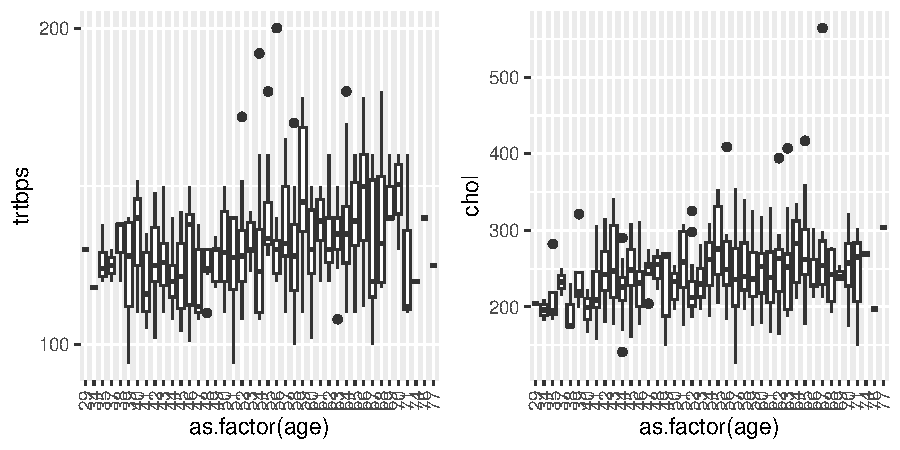
\includegraphics{coyolaf_ChristianOyola-PRA2_files/figure-latex/unnamed-chunk-7-1.pdf}

\begin{Shaded}
\begin{Highlighting}[]
\CommentTok{\# Crear el primer boxplot para \textquotesingle{}thalachh\textquotesingle{} en función de \textquotesingle{}age\textquotesingle{}}
\NormalTok{bp1 }\OtherTok{\textless{}{-}} \FunctionTok{ggplot}\NormalTok{(}\AttributeTok{data =}\NormalTok{ data\_heart, }\FunctionTok{aes}\NormalTok{(}\AttributeTok{x =} \FunctionTok{as.factor}\NormalTok{(age), }\AttributeTok{y =}\NormalTok{ thalachh)) }\SpecialCharTok{+} 
  \FunctionTok{geom\_boxplot}\NormalTok{() }\SpecialCharTok{+} \FunctionTok{scale\_y\_continuous}\NormalTok{(}\AttributeTok{breaks =} \FunctionTok{seq}\NormalTok{(}\AttributeTok{from =} \DecValTok{0}\NormalTok{, }\AttributeTok{to =} \DecValTok{1500}\NormalTok{, }\AttributeTok{by =} \DecValTok{100}\NormalTok{)) }\SpecialCharTok{+}
  \FunctionTok{theme}\NormalTok{(}\AttributeTok{axis.text.x =} \FunctionTok{element\_text}\NormalTok{(}\AttributeTok{angle =} \DecValTok{90}\NormalTok{, }\AttributeTok{vjust =} \FloatTok{0.5}\NormalTok{, }\AttributeTok{hjust=}\DecValTok{1}\NormalTok{))}
\CommentTok{\# Crear el segundo boxplot para \textquotesingle{}oldpeak\textquotesingle{} en función de \textquotesingle{}age\textquotesingle{}}
\NormalTok{bp2 }\OtherTok{\textless{}{-}} \FunctionTok{ggplot}\NormalTok{(}\AttributeTok{data =}\NormalTok{ data\_heart, }\FunctionTok{aes}\NormalTok{(}\AttributeTok{x =} \FunctionTok{as.factor}\NormalTok{(age), }\AttributeTok{y =}\NormalTok{ oldpeak)) }\SpecialCharTok{+} 
  \FunctionTok{geom\_boxplot}\NormalTok{() }\SpecialCharTok{+} \FunctionTok{scale\_y\_continuous}\NormalTok{(}\AttributeTok{breaks =} \FunctionTok{seq}\NormalTok{(}\AttributeTok{from =} \DecValTok{0}\NormalTok{, }\AttributeTok{to =} \DecValTok{1500}\NormalTok{, }\AttributeTok{by =} \DecValTok{100}\NormalTok{)) }\SpecialCharTok{+}
  \FunctionTok{theme}\NormalTok{(}\AttributeTok{axis.text.x =} \FunctionTok{element\_text}\NormalTok{(}\AttributeTok{angle =} \DecValTok{90}\NormalTok{, }\AttributeTok{vjust =} \FloatTok{0.5}\NormalTok{, }\AttributeTok{hjust=}\DecValTok{1}\NormalTok{))}
\FunctionTok{grid.arrange}\NormalTok{(bp1, bp2, }\AttributeTok{ncol =} \DecValTok{2}\NormalTok{)}
\end{Highlighting}
\end{Shaded}

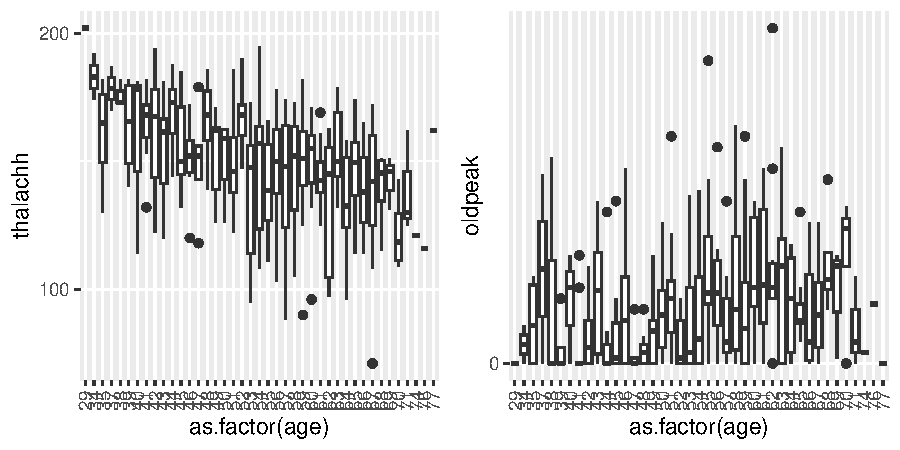
\includegraphics{coyolaf_ChristianOyola-PRA2_files/figure-latex/unnamed-chunk-8-1.pdf}

Tras este análisis, se llega a la conclusión de que es pertinente
incluir los valores atípicos (outliers) detectados en las variables en
el estudio. Esto se debe a que dichos valores podrían representar casos
clínicos atípicos, como episodios de hipertensión, o respuestas
inusuales frente a las mediciones. Se decide conservar estos valores
debido a la falta de información que confirme si son errores en la
entrada de datos o anomalías en las mediciones.

\hypertarget{anuxe1lisis-de-los-datos}{%
\subsection{2.4 Análisis de los datos}\label{anuxe1lisis-de-los-datos}}

Con la intención de tener un primer acercamiento con las variables y su
distribución, se empleará una representación gráfica basado en
histogramas:

\textbf{AGE}, \textbf{SEX}

\begin{Shaded}
\begin{Highlighting}[]
\CommentTok{\# Crear el primer gráfico (Histograma de Age)}
\NormalTok{p1 }\OtherTok{\textless{}{-}} \FunctionTok{ggplot}\NormalTok{(data\_heart, }\FunctionTok{aes}\NormalTok{(}\AttributeTok{x =}\NormalTok{ age)) }\SpecialCharTok{+}
  \FunctionTok{geom\_histogram}\NormalTok{(}\AttributeTok{color =} \StringTok{"black"}\NormalTok{) }\SpecialCharTok{+} \FunctionTok{ggtitle}\NormalTok{(}\StringTok{"Histograma de Age"}\NormalTok{)}
\CommentTok{\# Preparar los datos para el segundo gráfico (Histograma de Sex)}
\NormalTok{sex\_counts }\OtherTok{\textless{}{-}} \FunctionTok{table}\NormalTok{(data\_heart}\SpecialCharTok{$}\NormalTok{sex)}
\CommentTok{\# Crear el segundo gráfico (Histograma de Sex)}
\NormalTok{p2 }\OtherTok{\textless{}{-}} \FunctionTok{ggplot}\NormalTok{(}\FunctionTok{as.data.frame}\NormalTok{(sex\_counts), }\FunctionTok{aes}\NormalTok{(}\AttributeTok{x =}\NormalTok{ Var1, }\AttributeTok{y =}\NormalTok{ Freq)) }\SpecialCharTok{+}
  \FunctionTok{geom\_bar}\NormalTok{(}\AttributeTok{stat =} \StringTok{"identity"}\NormalTok{, }\AttributeTok{color =} \StringTok{"black"}\NormalTok{) }\SpecialCharTok{+}
  \FunctionTok{xlab}\NormalTok{(}\StringTok{"Sex"}\NormalTok{) }\SpecialCharTok{+} \FunctionTok{ylab}\NormalTok{(}\StringTok{"Count"}\NormalTok{) }\SpecialCharTok{+} \FunctionTok{ggtitle}\NormalTok{(}\StringTok{"Histograma de Sex"}\NormalTok{)}
\FunctionTok{grid.arrange}\NormalTok{(p1, p2, }\AttributeTok{ncol =} \DecValTok{2}\NormalTok{)}
\end{Highlighting}
\end{Shaded}

\begin{verbatim}
## `stat_bin()` using `bins = 30`. Pick better value with `binwidth`.
\end{verbatim}

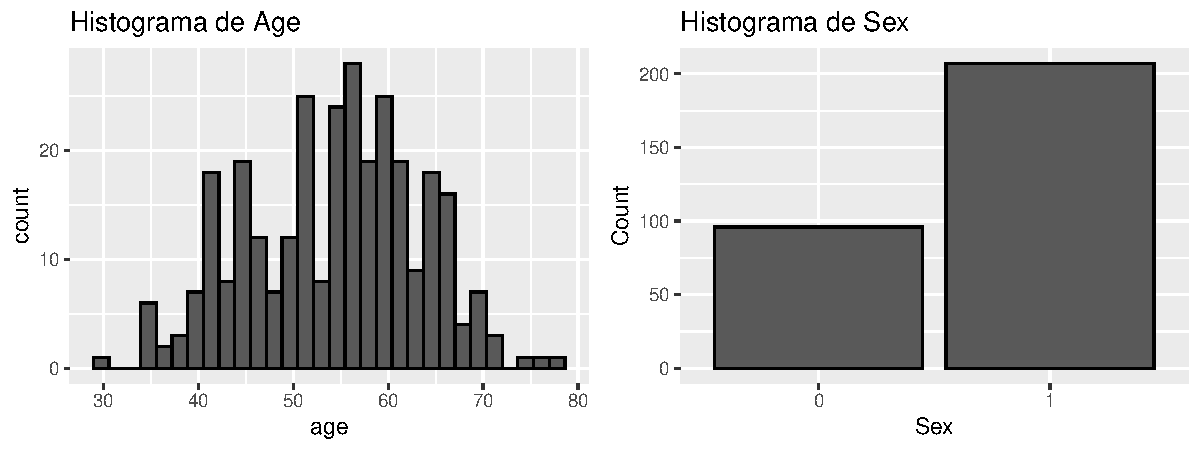
\includegraphics{coyolaf_ChristianOyola-PRA2_files/figure-latex/unnamed-chunk-9-1.pdf}

\textbf{AGE:} La distribución de las edades es multimodal, lo que
sugiere la presencia de varios grupos de edad distintos. Así mismo, se
identifica que la mayoría de los individuos en el conjunto de datos
están en sus 50 y 60 años. Hay menos individuos jóvenes y de avanzada
edad.

\textbf{SEX:} Esta distribución puede reflejar que los hombres están más
representados en los casos de ataques cardíacos dentro de la población
de datos, al rededor de 200 registros.

\textbf{CP, FBS}

\begin{Shaded}
\begin{Highlighting}[]
\NormalTok{cp\_counts }\OtherTok{\textless{}{-}} \FunctionTok{table}\NormalTok{(data\_heart}\SpecialCharTok{$}\NormalTok{cp)}
\NormalTok{p3 }\OtherTok{\textless{}{-}} \FunctionTok{ggplot}\NormalTok{() }\SpecialCharTok{+} \FunctionTok{geom\_bar}\NormalTok{(}\AttributeTok{data =} \FunctionTok{as.data.frame}\NormalTok{(cp\_counts), }\FunctionTok{aes}\NormalTok{(}\AttributeTok{x =}\NormalTok{ Var1, }\AttributeTok{y =}\NormalTok{ Freq), }
          \AttributeTok{stat =} \StringTok{"identity"}\NormalTok{, }\AttributeTok{color =} \StringTok{"black"}\NormalTok{) }\SpecialCharTok{+} \FunctionTok{xlab}\NormalTok{(}\StringTok{"CP"}\NormalTok{) }\SpecialCharTok{+} \FunctionTok{ylab}\NormalTok{(}\StringTok{"Count"}\NormalTok{) }\SpecialCharTok{+} 
  \FunctionTok{ggtitle}\NormalTok{(}\StringTok{"Histograma de CP"}\NormalTok{)}
\NormalTok{fbs\_counts }\OtherTok{\textless{}{-}} \FunctionTok{table}\NormalTok{(data\_heart}\SpecialCharTok{$}\NormalTok{fbs)}
\NormalTok{p4 }\OtherTok{\textless{}{-}} \FunctionTok{ggplot}\NormalTok{() }\SpecialCharTok{+} \FunctionTok{geom\_bar}\NormalTok{(}\AttributeTok{data =} \FunctionTok{as.data.frame}\NormalTok{(fbs\_counts), }\FunctionTok{aes}\NormalTok{(}\AttributeTok{x =}\NormalTok{ Var1, }\AttributeTok{y =}\NormalTok{ Freq), }
           \AttributeTok{stat =} \StringTok{"identity"}\NormalTok{, }\AttributeTok{color =} \StringTok{"black"}\NormalTok{) }\SpecialCharTok{+} \FunctionTok{xlab}\NormalTok{(}\StringTok{"FBS"}\NormalTok{) }\SpecialCharTok{+} \FunctionTok{ylab}\NormalTok{(}\StringTok{"Count"}\NormalTok{) }\SpecialCharTok{+} 
  \FunctionTok{ggtitle}\NormalTok{(}\StringTok{"Histograma de FBS"}\NormalTok{)}
\FunctionTok{grid.arrange}\NormalTok{(p3, p4, }\AttributeTok{ncol =} \DecValTok{2}\NormalTok{)}
\end{Highlighting}
\end{Shaded}

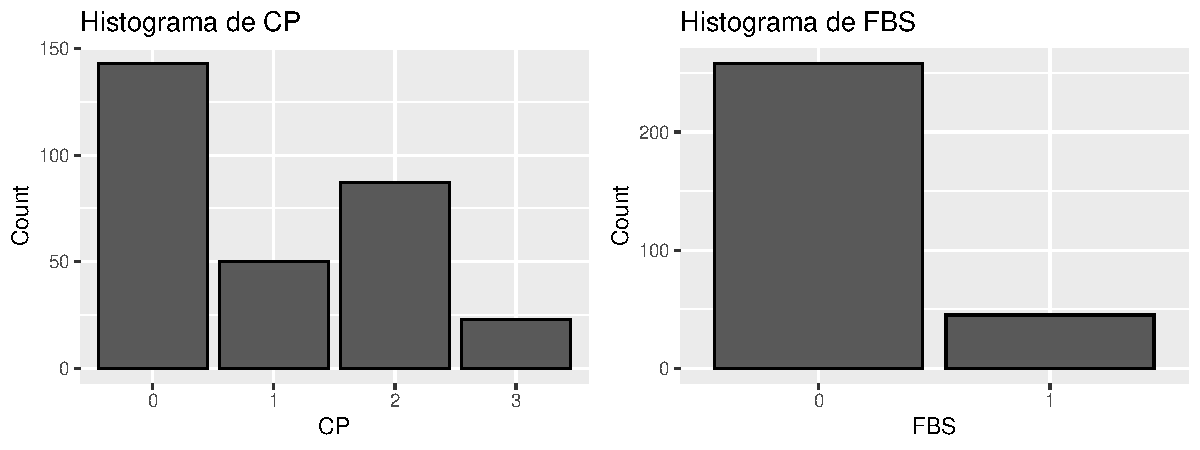
\includegraphics{coyolaf_ChristianOyola-PRA2_files/figure-latex/unnamed-chunk-10-1.pdf}

\textbf{CP:} A partir del análisis previo, se puede evidenciar que la
mayoría de las observaciones en el conjunto de datos corresponden a
individuos sin síntomas de dolor torácico. Las barras para `1' (angina
típica) y `2' (angina atípica) son más bajas, con `1' siendo la menos
común de las categorías sintomáticas. La categoría `3' (dolor no
anginoso) tiene la menor cantidad de observaciones.

\textbf{FBS:} Representa la distribución de los valores de glucosa en
sangre en ayunas: Categoría 0: Representa a los individuos con un nivel
de glucosa en sangre en ayunas de 120 mg/dl o menos. Categoría 1:
Representa a los individuos con un nivel de glucosa en sangre en ayunas
mayor de 120 mg/dl. Existe la presencia de más individuos con niveles
normales o bajos de glucosa en sangre en ayunas (\textless{} 120 mg/dl)
que aquellos con niveles altos (\textgreater{} 120 mg/dl), lo cual puede
ser relevante para la evaluación de riesgos cardíacos.

\textbf{TRTBPS, CHOL, THALACHH, OLDPEAK}

\begin{Shaded}
\begin{Highlighting}[]
\NormalTok{histList }\OtherTok{\textless{}{-}} \FunctionTok{list}\NormalTok{()}
\NormalTok{n }\OtherTok{=} \FunctionTok{c}\NormalTok{(}\StringTok{"trtbps"}\NormalTok{, }\StringTok{"chol"}\NormalTok{, }\StringTok{"thalachh"}\NormalTok{, }\StringTok{"oldpeak"}\NormalTok{)}
\NormalTok{datosAux }\OtherTok{=}\NormalTok{ data\_heart }\SpecialCharTok{\%\textgreater{}\%} \FunctionTok{select}\NormalTok{(}\FunctionTok{all\_of}\NormalTok{(n))}
\ControlFlowTok{for}\NormalTok{(y }\ControlFlowTok{in} \DecValTok{1}\SpecialCharTok{:}\FunctionTok{ncol}\NormalTok{(datosAux)) \{}
\NormalTok{  col }\OtherTok{\textless{}{-}} \FunctionTok{names}\NormalTok{(datosAux)[y]}
\NormalTok{  ggp }\OtherTok{\textless{}{-}} \FunctionTok{ggplot}\NormalTok{(datosAux, }\FunctionTok{aes\_string}\NormalTok{(}\AttributeTok{x =}\NormalTok{ col)) }\SpecialCharTok{+}
    \FunctionTok{geom\_histogram}\NormalTok{(}\AttributeTok{bins =} \DecValTok{30}\NormalTok{, }\AttributeTok{color =} \StringTok{"black"}\NormalTok{) }\SpecialCharTok{+}
    \FunctionTok{labs}\NormalTok{(}\AttributeTok{title =} \FunctionTok{paste}\NormalTok{(col))}
\NormalTok{  histList[[y]] }\OtherTok{\textless{}{-}}\NormalTok{ ggp }\CommentTok{\# Añadimos cada plot a la lista vacía}
\NormalTok{\}}
\FunctionTok{ggplot2.multiplot}\NormalTok{(}\AttributeTok{plotlist =}\NormalTok{ histList, }\AttributeTok{cols =} \DecValTok{2}\NormalTok{)}
\end{Highlighting}
\end{Shaded}

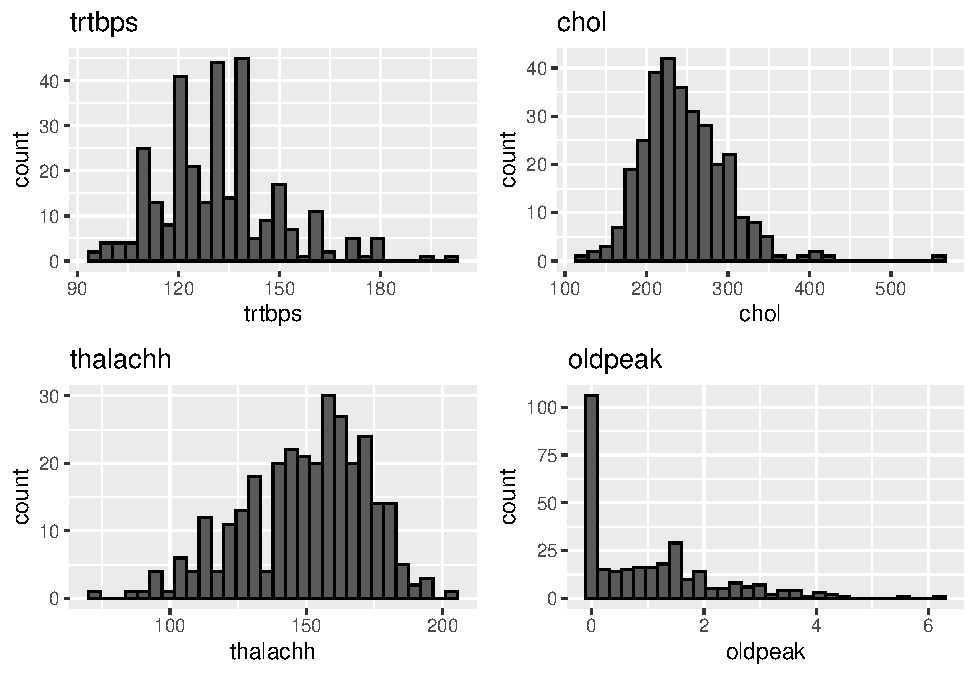
\includegraphics{coyolaf_ChristianOyola-PRA2_files/figure-latex/unnamed-chunk-11-1.pdf}

\textbf{TRTBPS:} Presión arterial en reposo (mmHg). La distribución
muestra varios picos, lo que puede indicar rangos comunes de presión
arterial en reposo o posibles agrupaciones de datos.

\textbf{CHOL:} Nivel de colesterol sérico (mg/dl). La distribución
parece aproximadamente normal con un pico central, indicando que la
mayoría de los individuos tienen niveles de colesterol en un rango
intermedio.

\textbf{THALACHH:} Máxima frecuencia cardíaca alcanzada. Esta
distribución también muestra una tendencia aproximadamente normal, con
la mayoría de los individuos alcanzando una frecuencia cardíaca máxima
en el rango medio.

\textbf{OLDPEAK:} Depresión del ST inducida por el ejercicio en relación
con el reposo. La distribución está sesgada hacia la izquierda, con la
mayoría de los individuos mostrando valores bajos de depresión del ST y
algunos pocos con valores más altos.

\textbf{RESTECG}

\begin{Shaded}
\begin{Highlighting}[]
\NormalTok{restecg\_counts }\OtherTok{\textless{}{-}} \FunctionTok{table}\NormalTok{(data\_heart}\SpecialCharTok{$}\NormalTok{restecg)}
\CommentTok{\# Histograma de los conteos de "restecg"}
\FunctionTok{ggplot}\NormalTok{() }\SpecialCharTok{+}
  \FunctionTok{geom\_bar}\NormalTok{(}\AttributeTok{data =} \FunctionTok{as.data.frame}\NormalTok{(restecg\_counts), }\FunctionTok{aes}\NormalTok{(}\AttributeTok{x =}\NormalTok{ Var1, }\AttributeTok{y =}\NormalTok{ Freq), }
           \AttributeTok{stat =} \StringTok{"identity"}\NormalTok{, }\AttributeTok{color =} \StringTok{"black"}\NormalTok{) }\SpecialCharTok{+}
  \FunctionTok{xlab}\NormalTok{(}\StringTok{"RESTECG"}\NormalTok{) }\SpecialCharTok{+}
  \FunctionTok{ylab}\NormalTok{(}\StringTok{"Count"}\NormalTok{) }\SpecialCharTok{+}
  \FunctionTok{ggtitle}\NormalTok{(}\StringTok{"Histograma de RESTECG"}\NormalTok{)}
\end{Highlighting}
\end{Shaded}

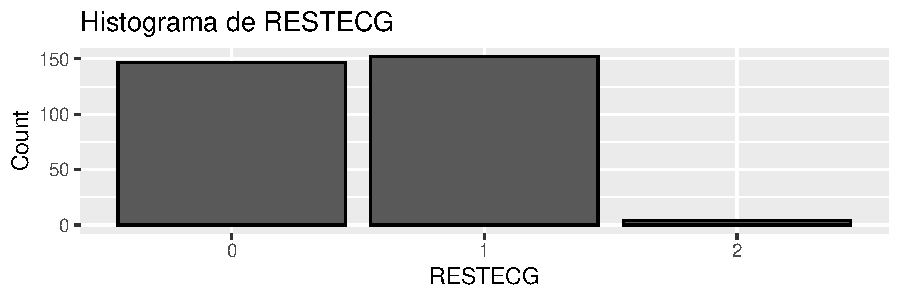
\includegraphics{coyolaf_ChristianOyola-PRA2_files/figure-latex/unnamed-chunk-12-1.pdf}

\textbf{RESTECG:} representa la distribución de los resultados
electrocardiográficos en reposo: 0: Normal, 1: Anormalidades en la onda
ST-T 2: Hipertrofia ventricular izquierda probable o definitiva. El
histograma indica que la cantidad de individuos con resultados ECG
normales y con anormalidades de onda ST-T es similar, mientras que
aquellos con hipertrofia ventricular izquierda son significativamente
menos en el conjunto de datos. Información relevante en la
identificación de enfermedades cardíacas.

\textbf{EXNG, SLP, CAA, THALL}

\begin{Shaded}
\begin{Highlighting}[]
\NormalTok{histList }\OtherTok{\textless{}{-}} \FunctionTok{list}\NormalTok{()}
\NormalTok{n }\OtherTok{=} \FunctionTok{c}\NormalTok{(}\StringTok{"exng"}\NormalTok{, }\StringTok{"slp"}\NormalTok{, }\StringTok{"caa"}\NormalTok{, }\StringTok{"thall"}\NormalTok{)}
\NormalTok{datosAux }\OtherTok{=}\NormalTok{ data\_heart }\SpecialCharTok{\%\textgreater{}\%} \FunctionTok{select}\NormalTok{(}\FunctionTok{all\_of}\NormalTok{(n))}
\ControlFlowTok{for}\NormalTok{(y }\ControlFlowTok{in} \DecValTok{1}\SpecialCharTok{:}\FunctionTok{ncol}\NormalTok{(datosAux)) \{}
\NormalTok{  col }\OtherTok{\textless{}{-}} \FunctionTok{names}\NormalTok{(datosAux)[y]}
\NormalTok{  ggp }\OtherTok{\textless{}{-}} \FunctionTok{ggplot}\NormalTok{(datosAux, }\FunctionTok{aes\_string}\NormalTok{(}\AttributeTok{x =}\NormalTok{ col)) }\SpecialCharTok{+}
    \FunctionTok{geom\_histogram}\NormalTok{(}\AttributeTok{bins =} \DecValTok{30}\NormalTok{, }\AttributeTok{color =} \StringTok{"black"}\NormalTok{) }\SpecialCharTok{+}
    \FunctionTok{labs}\NormalTok{(}\AttributeTok{title =} \FunctionTok{paste}\NormalTok{(}\StringTok{"Histograma"}\NormalTok{,col))}
\NormalTok{  histList[[y]] }\OtherTok{\textless{}{-}}\NormalTok{ ggp }\CommentTok{\# Añadimos cada plot a la lista vacía}
\NormalTok{\}}
\FunctionTok{ggplot2.multiplot}\NormalTok{(}\AttributeTok{plotlist =}\NormalTok{ histList, }\AttributeTok{cols =} \DecValTok{2}\NormalTok{)}
\end{Highlighting}
\end{Shaded}

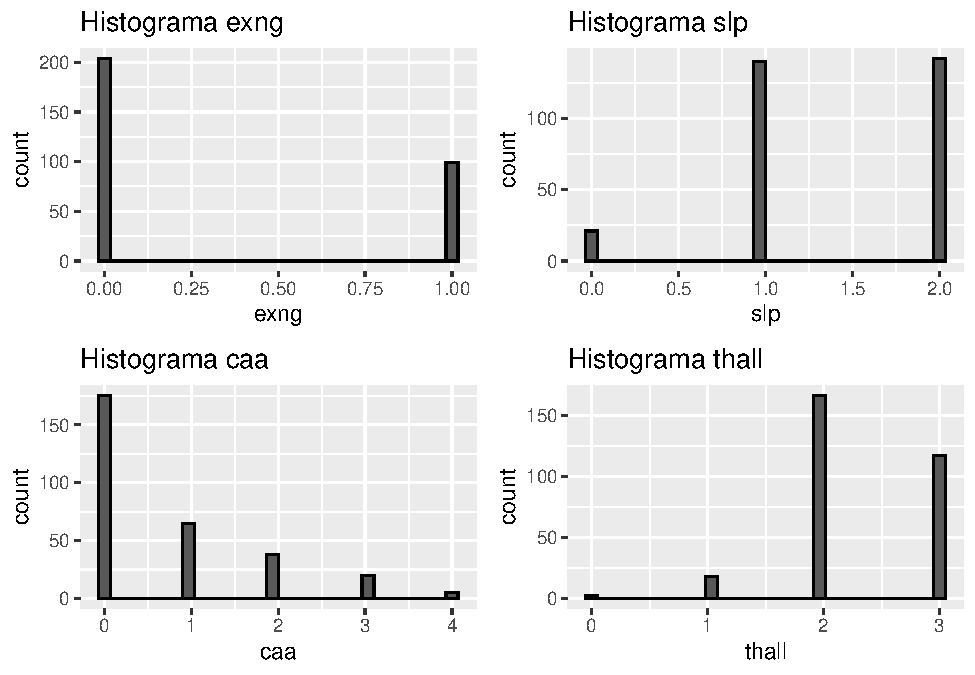
\includegraphics{coyolaf_ChristianOyola-PRA2_files/figure-latex/unnamed-chunk-13-1.pdf}

\textbf{exng (Angina inducida por ejercicio):} Se observan dos barras,
una para `0' (no) y otra para `1' (sí). La barra para `0' es más alta,
indicando que más individuos no experimentaron angina durante el
ejercicio.

\textbf{slp (Pendiente del segmento ST del ejercicio máximo):} Hay tres
barras, que corresponden a `0' (descendente), `1' (plano), y `2'
(ascendente). La pendiente plana es la más común, seguida por la
ascendente, y la descendente es la menos común.

\textbf{caa (Número de vasos principales coloreados por fluoroscopia):}
Las barras representan el conteo de vasos principales, desde `0' hasta
`3' o más. La mayoría de los individuos no tienen vasos coloreados
(barra `0'), y hay una disminución progresiva en el número a medida que
aumenta el número de vasos afectados.

\textbf{thall (Resultados de la prueba de talio):} Con barras para `1'
(defecto fijo), `2' (normal) y `3' (defecto reversible). La categoría
`2' (normal) es la más prevalente, seguida de la `3' (defecto
reversible), y la `1' (defecto fijo) es la menos común.

\hypertarget{comprobaciuxf3n-de-la-normalidad-y-homogeneidad-de-la-varianza.}{%
\subsubsection{2.4.1 Comprobación de la normalidad y homogeneidad de la
varianza.}\label{comprobaciuxf3n-de-la-normalidad-y-homogeneidad-de-la-varianza.}}

\begin{Shaded}
\begin{Highlighting}[]
\NormalTok{data\_heart}\SpecialCharTok{$}\NormalTok{output }\OtherTok{\textless{}{-}} \FunctionTok{as.factor}\NormalTok{(data\_heart}\SpecialCharTok{$}\NormalTok{output)}
\NormalTok{selected\_vars }\OtherTok{\textless{}{-}} \FunctionTok{c}\NormalTok{(}\StringTok{"age"}\NormalTok{, }\StringTok{"cp"}\NormalTok{, }\StringTok{"trtbps"}\NormalTok{, }\StringTok{"chol"}\NormalTok{, }\StringTok{"fbs"}\NormalTok{, }\StringTok{"restecg"}\NormalTok{, }\StringTok{"thalachh"}\NormalTok{, }\StringTok{"exng"}\NormalTok{, }
                   \StringTok{"oldpeak"}\NormalTok{, }\StringTok{"slp"}\NormalTok{, }\StringTok{"caa"}\NormalTok{, }\StringTok{"thall"}\NormalTok{)}
\CommentTok{\# Prueba de normalidad con la prueba de Shapiro{-}Wilk}
\NormalTok{normality\_tests }\OtherTok{\textless{}{-}} \FunctionTok{lapply}\NormalTok{(data\_heart[selected\_vars], shapiro.test)}
\CommentTok{\# dataframe para almacenar los resultados de la prueba de Shapiro{-}Wilk}
\NormalTok{normality\_results\_df }\OtherTok{\textless{}{-}} \FunctionTok{do.call}\NormalTok{(rbind, }\FunctionTok{lapply}\NormalTok{(normality\_tests, }\ControlFlowTok{function}\NormalTok{(test, var) \{}
  \FunctionTok{data.frame}\NormalTok{(}
    \AttributeTok{Variable =}\NormalTok{ var,}
    \AttributeTok{Shapiro\_W =}\NormalTok{ test}\SpecialCharTok{$}\NormalTok{statistic,}
    \AttributeTok{P\_Value =}\NormalTok{ test}\SpecialCharTok{$}\NormalTok{p.value}
\NormalTok{  )}
\NormalTok{\}, }\FunctionTok{names}\NormalTok{(normality\_tests)))}
\CommentTok{\# Prueba de homogeneidad de la varianza con la prueba de Levene}
\NormalTok{homogeneity\_tests }\OtherTok{\textless{}{-}} \FunctionTok{lapply}\NormalTok{(selected\_vars, }\ControlFlowTok{function}\NormalTok{(var) \{}
  \FunctionTok{leveneTest}\NormalTok{(}\FunctionTok{as.formula}\NormalTok{(}\FunctionTok{paste}\NormalTok{(var, }\StringTok{\textquotesingle{}\textasciitilde{} output\textquotesingle{}}\NormalTok{)), }\AttributeTok{data =}\NormalTok{ data\_heart)}
\NormalTok{\})}
\CommentTok{\# Mostramos los resultados de las pruebas de normalidad}
\FunctionTok{head}\NormalTok{(normality\_results\_df, }\DecValTok{4}\NormalTok{)}
\end{Highlighting}
\end{Shaded}

\begin{verbatim}
##       Variable Shapiro_W     P_Value
## age.1      age 0.9863705 0.005798359
## age.2       cp 0.9863705 0.005798359
## age.3   trtbps 0.9863705 0.005798359
## age.4     chol 0.9863705 0.005798359
\end{verbatim}

\begin{Shaded}
\begin{Highlighting}[]
\CommentTok{\# Mostramos los resultados de las pruebas de homogeneidad}
\CommentTok{\#print(homogeneity\_tests)}
\end{Highlighting}
\end{Shaded}

\textbf{Edad (age):} W = 0.98637, p-value = 0.005798 La distribución de
la edad no es normal al nivel de significancia estándar (p \textless{}
0.05).

\textbf{Tipo de dolor en el pecho (cp):} W = 0.79016, p-value
\textless{} 2.2e-16 La distribución de esta variable es
significativamente no normal.

\textbf{Presión arterial en reposo (trtbps):} W = 0.96592, p-value =
1.458e-06 La distribución de la presión arterial en reposo no es normal.

\textbf{Colesterol sérico (chol):} W = 0.94688, p-value = 5.365e-09 La
distribución del colesterol sérico no es normal.

\textbf{Azúcar en la sangre en ayunas (fbs):} W = 0.42399, p-value
\textless{} 2.2e-16 La distribución del azúcar en la sangre en ayunas es
significativamente no normal.

\textbf{Resultados electrocardiográficos en reposo (restecg):} W =
0.67932, p-value \textless{} 2.2e-16 La distribución de los resultados
del ECG en reposo no es normal.

\textbf{Máxima frecuencia cardíaca alcanzada (thalachh):} W = 0.97632,
p-value = 6.621e-05 La distribución de la frecuencia cardíaca máxima
alcanzada no es normal.

\textbf{Angina inducida por el ejercicio (exng):} W = 0.59126, p-value
\textless{} 2.2e-16 La distribución de la angina inducida por el
ejercicio es significativamente no normal.

\textbf{Depresión del ST inducida por el ejercicio (oldpeak):} W =
0.84418, p-value \textless{} 2.2e-16 La distribución de la depresión del
ST inducida por el ejercicio no es normal.

\textbf{Pendiente del segmento ST del ejercicio máximo (slp):} W =
0.74465, p-value \textless{} 2.2e-16 La distribución de la pendiente del
segmento ST no es normal.

\textbf{Número de vasos principales coloreados (caa):} W = 0.72812,
p-value \textless{} 2.2e-16 La distribución del número de vasos
principales coloreados no es normal.

\textbf{Defectos identificados en la prueba de talio (thall):} W =
0.75058, p-value \textless{} 2.2e-16 La distribución de los defectos
identificados en la prueba de talio no es normal.

La mayoría de las variables muestran p-valores significativamente
menores a 0.05, lo que indica que las distribuciones de estas variables
no son normales según la prueba de Shapiro-Wilk. Este es un hallazgo
importante que afecta la elección de las pruebas estadísticas a
utilizar; para datos no normales, se prefieren métodos no paramétricos.

\textbf{Age}: F = 7.9854, p-valor = 0.005031. La varianza no es
homogénea (p \textless{} 0.05). Hay una diferencia significativa en las
varianzas entre los grupos.

\textbf{Cp:} F = 12.158, p-valor = 0.0005617. La varianza no es
homogénea (p \textless{} 0.001). Existe una diferencia significativa en
las varianzas entre los grupos.

\textbf{Trtbps:} F = 1.857, p-valor = 0.174. Las varianzas son
homogéneas (p \textgreater{} 0.05). No hay una diferencia significativa
en las varianzas entre los grupos.

\textbf{Chol:} F = 0.1015, p-valor = 0.7503. Las varianzas son
homogéneas. No hay una diferencia significativa en las varianzas entre
los grupos.

\textbf{Fbs:} F = 0.2369, p-valor = 0.6268. Las varianzas son
homogéneas. No hay una diferencia significativa en las varianzas entre
los grupos.

\textbf{Restecg:} F = 0.2724, p-valor = 0.6021. Las varianzas son
homogéneas. No hay una diferencia significativa en las varianzas entre
los grupos.

\textbf{Thalachh:} F = 5.2467, p-valor = 0.02268. La varianza no es
homogénea (p \textless{} 0.05). Hay una diferencia significativa en las
varianzas entre los grupos.

\textbf{Exng:} F = 40.27, p-valor \textless{} 0.0001. La varianza no es
homogénea. Existe una diferencia significativa en las varianzas entre
los grupos.

\textbf{Oldpeak:} F = 32.916, p-valor \textless{} 0.0001. La varianza no
es homogénea. Existe una diferencia significativa en las varianzas entre
los grupos.

\textbf{Slp:} F = 1.0924, p-valor = 0.2968. Las varianzas son
homogéneas. No hay una diferencia significativa en las varianzas entre
los grupos.

\textbf{Caa:} F = 26.235, p-valor \textless{} 0.0001. La varianza no es
homogénea. Existe una diferencia significativa en las varianzas entre
los grupos.

\textbf{Thall:} F = 13.614, p-valor = 0.0002664. La varianza no es
homogénea. Existe una diferencia significativa en las varianzas entre
los grupos.

\hypertarget{dimensiuxf3n-demogruxe1fica-vs-dimensiuxf3n-anuxe1lisis-clinico}{%
\subsubsection{2.4.2 Dimensión demográfica vs Dimensión Análisis
Clinico}\label{dimensiuxf3n-demogruxe1fica-vs-dimensiuxf3n-anuxe1lisis-clinico}}

\textbf{AGE vs Dimensión Análisis Clinico}

Vamos a proceder a analizar la relación entre la variable AGE y la
Dimensión Análisis Clinico.

\begin{Shaded}
\begin{Highlighting}[]
\NormalTok{selected\_vars }\OtherTok{\textless{}{-}} \FunctionTok{c}\NormalTok{(}\StringTok{"cp"}\NormalTok{, }\StringTok{"trtbps"}\NormalTok{,  }\StringTok{"chol"}\NormalTok{, }\StringTok{"fbs"}\NormalTok{, }\StringTok{"restecg"}\NormalTok{, }\StringTok{"thalachh"}\NormalTok{, }\StringTok{"exng"}\NormalTok{, }\StringTok{"oldpeak"}\NormalTok{, }\StringTok{"slp"}\NormalTok{, }\StringTok{"caa"}\NormalTok{, }\StringTok{"thall"}\NormalTok{)}
\NormalTok{filtered\_data }\OtherTok{\textless{}{-}}\NormalTok{ data\_heart }\SpecialCharTok{\%\textgreater{}\%} \FunctionTok{select}\NormalTok{(age, }\FunctionTok{all\_of}\NormalTok{(selected\_vars))}
\CommentTok{\# Calculo correlaciones}
\NormalTok{correlations }\OtherTok{\textless{}{-}} \FunctionTok{sapply}\NormalTok{(filtered\_data[, }\SpecialCharTok{{-}}\DecValTok{1}\NormalTok{], }\ControlFlowTok{function}\NormalTok{(var) }\FunctionTok{cor}\NormalTok{(filtered\_data}\SpecialCharTok{$}\NormalTok{age, var))}
\NormalTok{correlations}
\end{Highlighting}
\end{Shaded}

\begin{verbatim}
##          cp      trtbps        chol         fbs     restecg    thalachh 
## -0.06865302  0.27935091  0.21367796  0.12130765 -0.11621090 -0.39852194 
##        exng     oldpeak         slp         caa       thall 
##  0.09680083  0.21001257 -0.16881424  0.27632624  0.06800138
\end{verbatim}

\begin{Shaded}
\begin{Highlighting}[]
\NormalTok{first\_half\_vars }\OtherTok{\textless{}{-}}\NormalTok{ selected\_vars[}\DecValTok{1}\SpecialCharTok{:}\DecValTok{5}\NormalTok{]}
\NormalTok{second\_half\_vars }\OtherTok{\textless{}{-}}\NormalTok{ selected\_vars[}\DecValTok{6}\SpecialCharTok{:}\DecValTok{11}\NormalTok{]}
\NormalTok{first\_half\_graphList }\OtherTok{\textless{}{-}} \FunctionTok{vector}\NormalTok{(}\StringTok{\textquotesingle{}list\textquotesingle{}}\NormalTok{, }\FunctionTok{length}\NormalTok{(first\_half\_vars))}
\NormalTok{second\_half\_graphList }\OtherTok{\textless{}{-}} \FunctionTok{vector}\NormalTok{(}\StringTok{\textquotesingle{}list\textquotesingle{}}\NormalTok{, }\FunctionTok{length}\NormalTok{(second\_half\_vars))}
\NormalTok{create\_graphs }\OtherTok{\textless{}{-}} \ControlFlowTok{function}\NormalTok{(vars, graphList) \{}
  \ControlFlowTok{for}\NormalTok{ (i }\ControlFlowTok{in} \FunctionTok{seq\_along}\NormalTok{(vars)) \{}
\NormalTok{    var }\OtherTok{\textless{}{-}}\NormalTok{ vars[i]}
\NormalTok{    graphList[[i]] }\OtherTok{\textless{}{-}} \FunctionTok{ggplot}\NormalTok{(}\AttributeTok{data =}\NormalTok{ data\_heart, }\FunctionTok{aes\_string}\NormalTok{(}\AttributeTok{x =} \StringTok{"age"}\NormalTok{, }\AttributeTok{y =}\NormalTok{ var)) }\SpecialCharTok{+}
      \FunctionTok{geom\_point}\NormalTok{(}\AttributeTok{color =} \StringTok{"gray30"}\NormalTok{) }\SpecialCharTok{+} \FunctionTok{geom\_smooth}\NormalTok{(}\AttributeTok{method =} \StringTok{"lm"}\NormalTok{, }\AttributeTok{color =} \StringTok{"cornflowerblue"}\NormalTok{, }\AttributeTok{se =} \ConstantTok{FALSE}\NormalTok{) }\SpecialCharTok{+}
      \FunctionTok{labs}\NormalTok{(}\AttributeTok{x =} \StringTok{"Age"}\NormalTok{, }\AttributeTok{y =}\NormalTok{ var) }\SpecialCharTok{+} \FunctionTok{theme\_bw}\NormalTok{()}
\NormalTok{  \}}
  \FunctionTok{return}\NormalTok{(graphList)}
\NormalTok{\}}
\NormalTok{first\_half\_graphList }\OtherTok{\textless{}{-}} \FunctionTok{create\_graphs}\NormalTok{(first\_half\_vars, first\_half\_graphList)}
\NormalTok{second\_half\_graphList }\OtherTok{\textless{}{-}} \FunctionTok{create\_graphs}\NormalTok{(second\_half\_vars, second\_half\_graphList)}
\FunctionTok{grid.arrange}\NormalTok{(}\AttributeTok{grobs =}\NormalTok{ first\_half\_graphList, }\AttributeTok{ncol =} \DecValTok{2}\NormalTok{)}
\end{Highlighting}
\end{Shaded}

\begin{verbatim}
## `geom_smooth()` using formula = 'y ~ x'
## `geom_smooth()` using formula = 'y ~ x'
## `geom_smooth()` using formula = 'y ~ x'
## `geom_smooth()` using formula = 'y ~ x'
## `geom_smooth()` using formula = 'y ~ x'
\end{verbatim}

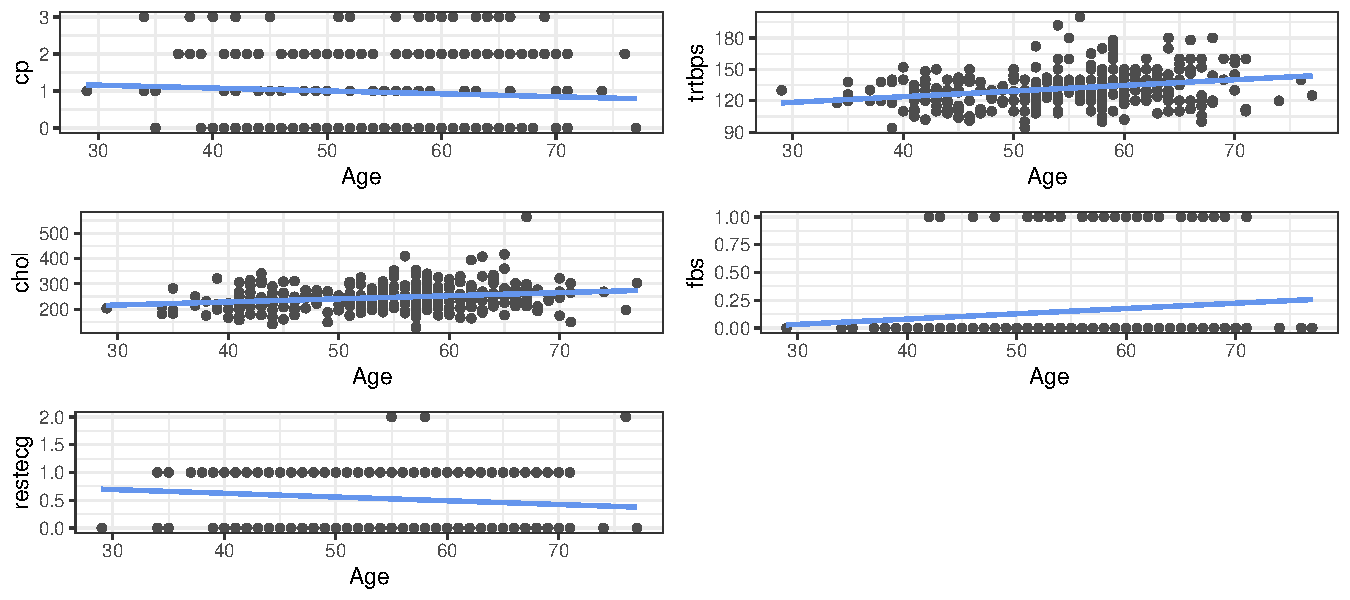
\includegraphics{coyolaf_ChristianOyola-PRA2_files/figure-latex/unnamed-chunk-16-1.pdf}

\begin{itemize}
\item
  \textbf{cp (dolor en el pecho):} Con un coeficiente de -0.06865302,
  hay una correlación negativa muy débil con la edad, lo que sugiere que
  no hay una relación lineal significativa entre la edad y el tipo de
  dolor en el pecho experimentado.
\item
  \textbf{trtbps (presión arterial en reposo):} El coeficiente de
  0.27935091, correlación positiva débil a moderada con la edad, lo que
  significa que la presión arterial en reposo tiende a aumentar
  ligeramente a medida que la gente envejece.
\item
  \textbf{chol (colesterol sérico):} Una correlación de 0.21367796
  positiva entre el nivel de colesterol y la edad, lo que podría indicar
  que los niveles de colesterol tienden a ser más altos en individuos de
  mayor edad.
\item
  \textbf{fbs (azúcar en la sangre en ayunas):} Con un coeficiente de
  0.12130765, hay una correlación positiva muy débil, lo que sugiere que
  hay poca o ninguna relación lineal directa entre la edad y los niveles
  de azúcar en la sangre en ayunas.
\item
  \textbf{restecg (electrocardiográficos en reposo):} El valor de
  -0.11621090, una correlación negativa muy débil con la edad,
  implicando que no hay una relación lineal clara entre los resultados
  del ECG en reposo y la edad.
\end{itemize}

\begin{Shaded}
\begin{Highlighting}[]
\FunctionTok{grid.arrange}\NormalTok{(}\AttributeTok{grobs =}\NormalTok{ second\_half\_graphList, }\AttributeTok{ncol =} \DecValTok{2}\NormalTok{)}
\end{Highlighting}
\end{Shaded}

\begin{verbatim}
## `geom_smooth()` using formula = 'y ~ x'
## `geom_smooth()` using formula = 'y ~ x'
## `geom_smooth()` using formula = 'y ~ x'
## `geom_smooth()` using formula = 'y ~ x'
## `geom_smooth()` using formula = 'y ~ x'
## `geom_smooth()` using formula = 'y ~ x'
\end{verbatim}

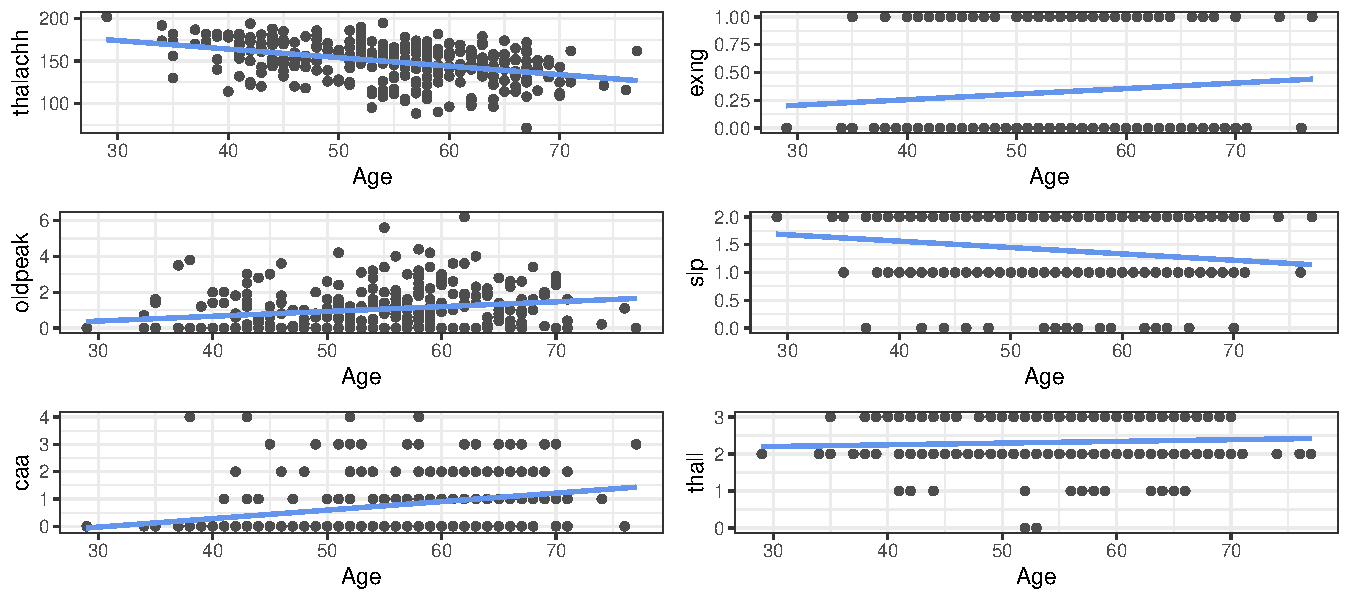
\includegraphics{coyolaf_ChristianOyola-PRA2_files/figure-latex/unnamed-chunk-17-1.pdf}

\begin{itemize}
\item
  \textbf{thalachh (máxima frecuencia cardíaca alcanzada):} Una
  correlación negativa -0.39852194 indica que a medida que la edad
  aumenta, la frecuencia cardíaca máxima alcanzada tiende a disminuir.
\item
  \textbf{exng (angina inducida por el ejercicio):} La correlación
  positiva de 0.09680083 indica que no hay una relación lineal
  significativa entre la angina inducida por el ejercicio y la edad.
\item
  \textbf{oldpeak (depresión del ST inducida por el ejercicio en
  relación con el reposo):} Con un coeficiente de 0.21001257, hay una
  correlación positiva débil, lo que podría significar que hay una leve
  tendencia a que la depresión del ST sea mayor en personas de mayor
  edad.
\item
  \textbf{slp (la pendiente del segmento ST del ejercicio máximo):} El
  valor de -0.16881424 muestra una correlación negativa débil,
  sugiriendo que la pendiente del segmento ST durante el ejercicio
  máximo tiende a disminuir ligeramente con la edad.
\item
  \textbf{caa (número de vasos principales coloreados por
  fluoroscopia):} Una correlación de 0.27632624 indica una relación
  positiva débil a moderada con la edad, lo que podría implicar que la
  probabilidad de tener una mayor cantidad de vasos coloreados aumenta
  con la edad.
\item
  \textbf{thall (defectos identificados en la prueba de talio):} La
  correlación positiva muy débil de 0.06800138 sugiere que apenas hay
  una relación entre los defectos detectados por la prueba de talio y la
  edad.
\end{itemize}

\hypertarget{genero-vs-dimensiuxf3n-laboratorio}{%
\subsubsection{2.4.3 Genero vs Dimensión
laboratorio}\label{genero-vs-dimensiuxf3n-laboratorio}}

Vamos a proceder a analizar la relación entre la variable de genero y la
Dimensión laboratorio.

\begin{Shaded}
\begin{Highlighting}[]
\NormalTok{data\_heart}\SpecialCharTok{$}\NormalTok{sex }\OtherTok{\textless{}{-}} \FunctionTok{factor}\NormalTok{(data\_heart}\SpecialCharTok{$}\NormalTok{sex, }\AttributeTok{levels =} \FunctionTok{c}\NormalTok{(}\DecValTok{0}\NormalTok{, }\DecValTok{1}\NormalTok{), }\AttributeTok{labels =} \FunctionTok{c}\NormalTok{(}\StringTok{"Femenino"}\NormalTok{, }\StringTok{"Masculino"}\NormalTok{))}
\NormalTok{selected\_vars }\OtherTok{\textless{}{-}} \FunctionTok{c}\NormalTok{(}\StringTok{"cp"}\NormalTok{, }\StringTok{"trtbps"}\NormalTok{, }\StringTok{"chol"}\NormalTok{, }\StringTok{"fbs"}\NormalTok{, }\StringTok{"restecg"}\NormalTok{, }\StringTok{"thalachh"}\NormalTok{, }\StringTok{"exng"}\NormalTok{, }\StringTok{"oldpeak"}\NormalTok{, }\StringTok{"slp"}\NormalTok{, }\StringTok{"caa"}\NormalTok{, }\StringTok{"thall"}\NormalTok{)}
\NormalTok{filtered\_data }\OtherTok{\textless{}{-}}\NormalTok{ data\_heart }\SpecialCharTok{\%\textgreater{}\%} \FunctionTok{select}\NormalTok{(sex, }\FunctionTok{all\_of}\NormalTok{(selected\_vars))}
\NormalTok{first\_group\_vars }\OtherTok{\textless{}{-}}\NormalTok{ selected\_vars[}\DecValTok{1}\SpecialCharTok{:}\DecValTok{5}\NormalTok{]}
\NormalTok{second\_group\_vars }\OtherTok{\textless{}{-}}\NormalTok{ selected\_vars[}\DecValTok{6}\SpecialCharTok{:}\DecValTok{11}\NormalTok{]}
\NormalTok{hist\_list }\OtherTok{\textless{}{-}} \FunctionTok{lapply}\NormalTok{(first\_group\_vars, }\ControlFlowTok{function}\NormalTok{(var) \{}
  \FunctionTok{ggplot}\NormalTok{(filtered\_data, }\FunctionTok{aes\_string}\NormalTok{(}\AttributeTok{x =}\NormalTok{ var, }\AttributeTok{fill =} \StringTok{"sex"}\NormalTok{)) }\SpecialCharTok{+}
    \FunctionTok{geom\_histogram}\NormalTok{(}\AttributeTok{data =} \FunctionTok{subset}\NormalTok{(filtered\_data, sex }\SpecialCharTok{==} \StringTok{"Masculino"}\NormalTok{), }\AttributeTok{bins =} \DecValTok{30}\NormalTok{, }\AttributeTok{alpha =} \FloatTok{0.5}\NormalTok{) }\SpecialCharTok{+}
    \FunctionTok{geom\_histogram}\NormalTok{(}\AttributeTok{data =} \FunctionTok{subset}\NormalTok{(filtered\_data, sex }\SpecialCharTok{==} \StringTok{"Femenino"}\NormalTok{), }\AttributeTok{bins =} \DecValTok{30}\NormalTok{, }\AttributeTok{alpha =} \FloatTok{0.7}\NormalTok{) }\SpecialCharTok{+}
    \FunctionTok{scale\_fill\_manual}\NormalTok{(}\AttributeTok{values =} \FunctionTok{c}\NormalTok{(}\StringTok{"Femenino"} \OtherTok{=} \StringTok{"orange"}\NormalTok{, }\StringTok{"Masculino"} \OtherTok{=} \StringTok{"blue"}\NormalTok{)) }\SpecialCharTok{+}
    \FunctionTok{labs}\NormalTok{(}\AttributeTok{x =}\NormalTok{ var, }\AttributeTok{y =} \StringTok{"Count"}\NormalTok{, }\AttributeTok{fill =} \StringTok{"Género"}\NormalTok{) }\SpecialCharTok{+} \FunctionTok{ggtitle}\NormalTok{(}\FunctionTok{paste}\NormalTok{(}\StringTok{"Histograma de"}\NormalTok{, var, }\StringTok{"por Género"}\NormalTok{)) }\SpecialCharTok{+} \FunctionTok{theme\_minimal}\NormalTok{()}
\NormalTok{\}) }
\NormalTok{first\_group\_grid }\OtherTok{\textless{}{-}} \FunctionTok{do.call}\NormalTok{(grid.arrange, }\FunctionTok{c}\NormalTok{(hist\_list, }\AttributeTok{ncol =} \DecValTok{2}\NormalTok{))}
\end{Highlighting}
\end{Shaded}

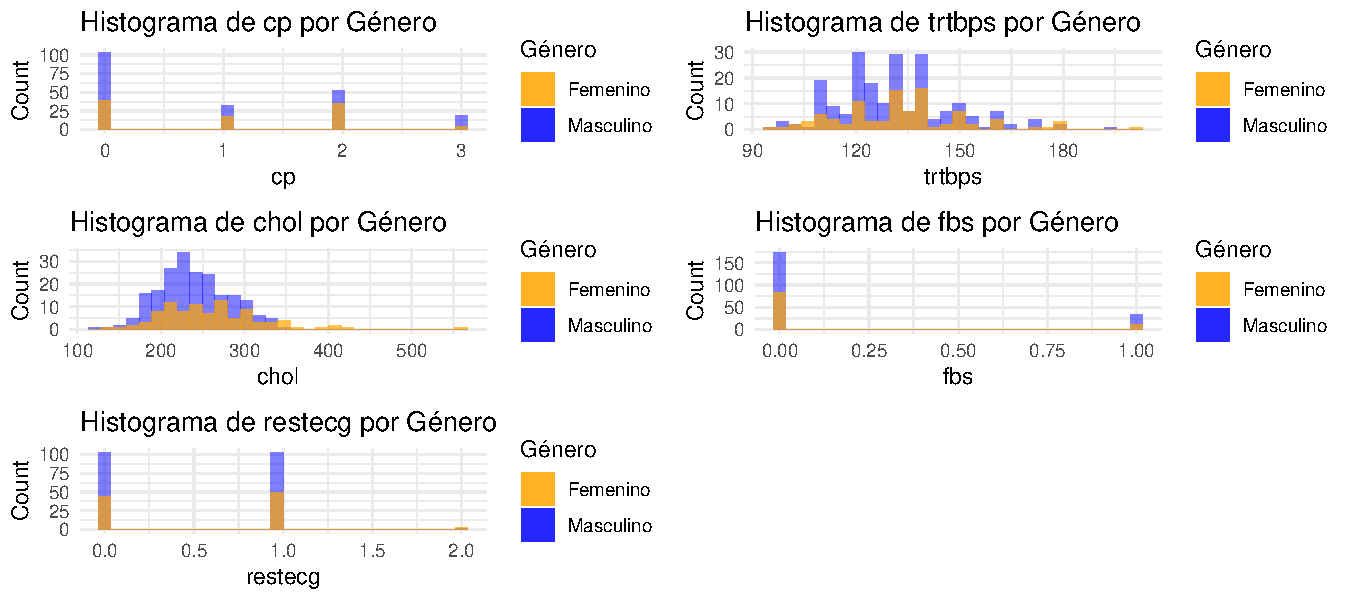
\includegraphics{coyolaf_ChristianOyola-PRA2_files/figure-latex/unnamed-chunk-18-1.pdf}

\begin{itemize}
\item
  \textbf{Distribución de cp (dolor en el pecho):} La mayoría de los
  individuos, parecen tener un tipo de dolor en el pecho tipo `0', lo
  que podría indicar el tipo más común en el conjunto de Datos. Hay
  menos incidencias de las categorías `1', `2' y `3', con los hombres
  mostrando ligeramente más casos en estas categorías que las mujeres.
\item
  \textbf{Distribución de trtbps (presión arterial en reposo):} La
  distribución de la presión arterial en reposo para los hombres muestra
  una tendencia a valores más altos en comparación con las mujeres.
  Ambos presentan un pico al rededor de los 120-140 mmHg, que está en el
  rango de la presión arterial normal.
\item
  \textbf{Distribución de chol (colesterol sérico):} Tanto hombres como
  mujeres presentan una distribución similar del colesterol sérico, con
  un pico claro alrededor de 200-250 mg/dl. Esto sugiere que la mayoría
  de los individuos en la muestra tienen niveles de colesterol dentro de
  lo que se consideraría un rango normal o ligeramente elevado.
\item
  \textbf{Distribución de fbs (azúcar en la sangre en ayunas):} La gran
  mayoría de los individuos de ambos géneros tienen un azúcar en la
  sangre en ayunas inferior a 0.25, lo que probablemente indica niveles
  normales de glucosa en ayunas.
\item
  \textbf{Distribución de restecg (resultados electrocardiográficos en
  reposo):} La categoría `0' y '1, son las más comúnes para los
  resultados del ECG en reposo en ambos géneros, lo que podría indicar
  una presencia de hipertrofia y una ausencia general de anomalías
  notables en el ECG de la mayoría de la muestra.
\end{itemize}

\begin{Shaded}
\begin{Highlighting}[]
\NormalTok{hist\_list }\OtherTok{\textless{}{-}} \FunctionTok{lapply}\NormalTok{(second\_group\_vars, }\ControlFlowTok{function}\NormalTok{(var) \{}
  \FunctionTok{ggplot}\NormalTok{(filtered\_data, }\FunctionTok{aes\_string}\NormalTok{(}\AttributeTok{x =}\NormalTok{ var, }\AttributeTok{fill =} \StringTok{"sex"}\NormalTok{)) }\SpecialCharTok{+}
    \FunctionTok{geom\_histogram}\NormalTok{(}\AttributeTok{data =} \FunctionTok{subset}\NormalTok{(filtered\_data, sex }\SpecialCharTok{==} \StringTok{"Masculino"}\NormalTok{), }\AttributeTok{bins =} \DecValTok{30}\NormalTok{, }\AttributeTok{alpha =} \FloatTok{0.5}\NormalTok{) }\SpecialCharTok{+}
    \FunctionTok{geom\_histogram}\NormalTok{(}\AttributeTok{data =} \FunctionTok{subset}\NormalTok{(filtered\_data, sex }\SpecialCharTok{==} \StringTok{"Femenino"}\NormalTok{), }\AttributeTok{bins =} \DecValTok{30}\NormalTok{, }\AttributeTok{alpha =} \FloatTok{0.7}\NormalTok{) }\SpecialCharTok{+}
    \FunctionTok{scale\_fill\_manual}\NormalTok{(}\AttributeTok{values =} \FunctionTok{c}\NormalTok{(}\StringTok{"Femenino"} \OtherTok{=} \StringTok{"orange"}\NormalTok{, }\StringTok{"Masculino"} \OtherTok{=} \StringTok{"blue"}\NormalTok{)) }\SpecialCharTok{+}
    \FunctionTok{labs}\NormalTok{(}\AttributeTok{x =}\NormalTok{ var, }\AttributeTok{y =} \StringTok{"Count"}\NormalTok{, }\AttributeTok{fill =} \StringTok{"Género"}\NormalTok{) }\SpecialCharTok{+} \FunctionTok{ggtitle}\NormalTok{(}\FunctionTok{paste}\NormalTok{(}\StringTok{"Histograma de"}\NormalTok{, var, }\StringTok{"por Género"}\NormalTok{)) }\SpecialCharTok{+}  \FunctionTok{theme\_minimal}\NormalTok{()\}) }
\NormalTok{second\_group\_grid }\OtherTok{\textless{}{-}} \FunctionTok{do.call}\NormalTok{(grid.arrange, }\FunctionTok{c}\NormalTok{(hist\_list, }\AttributeTok{ncol =} \DecValTok{2}\NormalTok{))}
\end{Highlighting}
\end{Shaded}

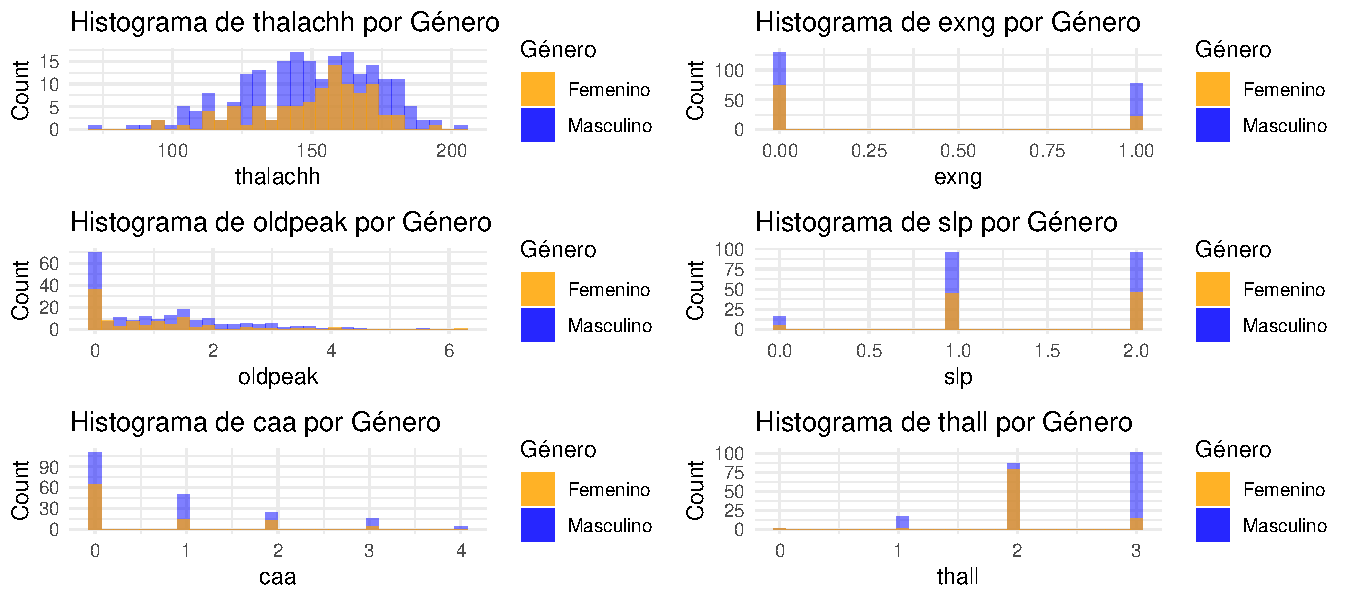
\includegraphics{coyolaf_ChristianOyola-PRA2_files/figure-latex/unnamed-chunk-19-1.pdf}

\begin{itemize}
\item
  \textbf{Distribución de thalachh (máxima frecuencia cardíaca
  alcanzada):}Ambos géneros muestran una distribución similar con un
  pico en la frecuencia cardíaca alrededor de 150 a 160 bpm (latidos por
  minuto). Los hombres tienden a tener un rango ligeramente más amplio
  de frecuencias cardíacas máximas comparado con las mujeres.
\item
  \textbf{Distribución de exng (angina inducida por el ejercicio):} La
  mayoría de los individuos en ambos géneros no experimentan angina
  inducida por el ejercicio, como se muestra por las barras altas en la
  categoría `0'.
\item
  \textbf{Distribución de oldpeak (depresión del ST inducida por el
  ejercicio en relación con el reposo):} Los valores de `oldpeak' para
  ambos géneros están mayormente concentrados cerca de 0, lo que indica
  que la muestra o de los sujetos no tienen una significativa depresión
  del segmento ST. Hay algunos casos, más visible en hombres, donde su
  valor de `oldpeak' es mayor, lo que podría indicar algún grado de
  enfermedad relacionada con el corazón.
\item
  \textbf{Distribución de slp (la pendiente del segmento ST del
  ejercicio máximo):} La pendiente del segmento ST parece ser más
  comúnmente de tipo `2' para ambos géneros, lo cual puede considerarse
  como normal.
\item
  \textbf{Distribución de caa (número de vasos principales coloreados
  por fluoroscopia):} La mayoría de los sujetos de ambos géneros parecen
  no tener vasos principales coloreados (categoría `0'), lo que podría
  ser indicativo de ausencia de enfermedad relacionada con el corazón
  relevante. Hay una presencia notable de individuos masculinos con
  mayor número de vasos coloreados en comparación con las mujeres.
\item
  \textbf{Distribución de thall (defectos identificados en la prueba de
  talio):} La categoría `2' parece ser la más prevalente en hombres y
  mujeres, lo que podría corresponder a un hallazgo normal o a la
  ausencia de defectos reversibles en la prueba de talio. Hay menos
  casos en las categorías `1' y `3', con los hombres mostrando una
  distribución más amplia entre estas categorías en comparación con las
  mujeres.
\end{itemize}

\hypertarget{relaciuxf3n-entre-variables}{%
\subsubsection{2.4.4 Relación entre
variables}\label{relaciuxf3n-entre-variables}}

Vamos a buscar las relaciones en función de la variable OUTPUT y unas
variables elegidas que creemos que pueden ayudar a predecir los
inconvenientes de ataque al corazón:

Debido a que dentro de OUTPUT, cada clase tiene una representación
notablemente distinta, realizaremos un analisis mediante gráficos de
densidad:

\begin{Shaded}
\begin{Highlighting}[]
\CommentTok{\# Ajustar el factor de la variable CLASS con los nombres de etiquetas deseadas}
\NormalTok{data\_heart}\SpecialCharTok{$}\NormalTok{output }\OtherTok{\textless{}{-}} \FunctionTok{factor}\NormalTok{(data\_heart}\SpecialCharTok{$}\NormalTok{output, }\AttributeTok{levels =} \FunctionTok{c}\NormalTok{(}\StringTok{"1"}\NormalTok{, }\StringTok{"0"}\NormalTok{),}
                      \AttributeTok{labels =} \FunctionTok{c}\NormalTok{(}\StringTok{"heart{-}attack"}\NormalTok{, }\StringTok{"no{-}heart{-}attack"}\NormalTok{))}
\CommentTok{\# Variables seleccionadas}
\NormalTok{selected\_vars }\OtherTok{\textless{}{-}} \FunctionTok{c}\NormalTok{(}\StringTok{"age"}\NormalTok{, }\StringTok{"cp"}\NormalTok{, }\StringTok{"trtbps"}\NormalTok{, }\StringTok{"chol"}\NormalTok{, }\StringTok{"fbs"}\NormalTok{, }\StringTok{"restecg"}\NormalTok{, }\StringTok{"thalachh"}\NormalTok{, }\StringTok{"exng"}\NormalTok{, }\StringTok{"oldpeak"}\NormalTok{, }\StringTok{"slp"}\NormalTok{, }\StringTok{"caa"}\NormalTok{, }\StringTok{"thall"}\NormalTok{)}
\CommentTok{\# Crear el grid de gráficos de densidad}
\FunctionTok{ggplot}\NormalTok{(data\_heart, }\FunctionTok{aes}\NormalTok{(}\AttributeTok{fill =}\NormalTok{ output)) }\SpecialCharTok{+}
  \FunctionTok{facet\_wrap}\NormalTok{(}\SpecialCharTok{\textasciitilde{}}\NormalTok{ variable, }\AttributeTok{scales =} \StringTok{"free"}\NormalTok{, }\AttributeTok{nrow =} \DecValTok{2}\NormalTok{) }\SpecialCharTok{+}
  \FunctionTok{geom\_density}\NormalTok{(}\AttributeTok{data =}\NormalTok{ reshape2}\SpecialCharTok{::}\FunctionTok{melt}\NormalTok{(data\_heart, }\AttributeTok{id.vars =} \StringTok{"output"}\NormalTok{, }\AttributeTok{measure.vars =}\NormalTok{ selected\_vars),}
               \FunctionTok{aes}\NormalTok{(}\AttributeTok{x =}\NormalTok{ value, }\AttributeTok{color =}\NormalTok{ output), }\AttributeTok{alpha =} \FloatTok{0.5}\NormalTok{) }\SpecialCharTok{+}
  \FunctionTok{labs}\NormalTok{(}\AttributeTok{x =} \StringTok{""}\NormalTok{, }\AttributeTok{y =} \StringTok{"Densidad"}\NormalTok{, }\AttributeTok{fill =} \StringTok{"output"}\NormalTok{) }\SpecialCharTok{+}
  \FunctionTok{scale\_fill\_manual}\NormalTok{(}\AttributeTok{values =} \FunctionTok{c}\NormalTok{(}\StringTok{"heart{-}attack"} \OtherTok{=} \StringTok{"red"}\NormalTok{, }\StringTok{"no{-}heart{-}attack"} \OtherTok{=} \StringTok{"blue"}\NormalTok{)) }\SpecialCharTok{+}
  \FunctionTok{scale\_color\_manual}\NormalTok{(}\AttributeTok{values =} \FunctionTok{c}\NormalTok{(}\StringTok{"heart{-}attack"} \OtherTok{=} \StringTok{"red"}\NormalTok{, }\StringTok{"no{-}heart{-}attack"} \OtherTok{=} \StringTok{"blue"}\NormalTok{)) }\SpecialCharTok{+}
  \FunctionTok{theme\_minimal}\NormalTok{()}
\end{Highlighting}
\end{Shaded}

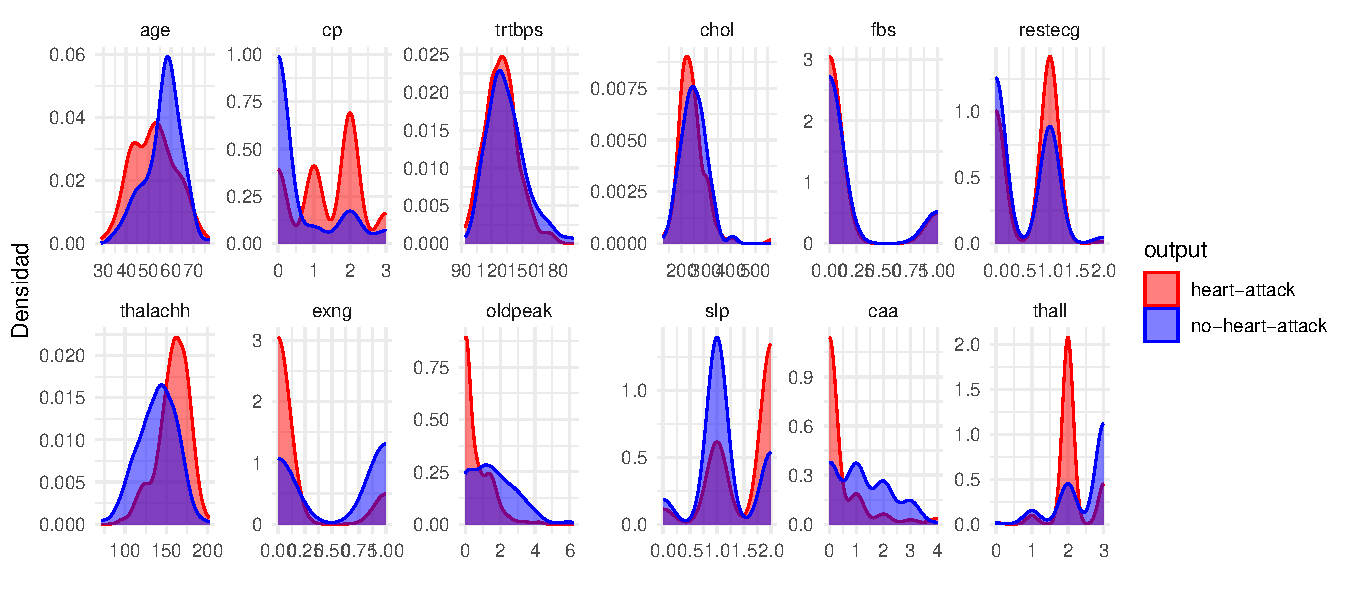
\includegraphics{coyolaf_ChristianOyola-PRA2_files/figure-latex/unnamed-chunk-20-1.pdf}

\begin{itemize}
\item
  \textbf{Edad (age):} Los pacientes que han sufrido un ataque cardíaco
  tienden a ser mayores en comparación con aquellos que no han sufrido
  uno, como lo indica la curva roja desplazada hacia la derecha.
\item
  \textbf{Presión arterial en reposo (trtbps):} La presión arterial en
  reposo de los pacientes que han sufrido un ataque cardíaco parece
  tener una distribución similar a la de aquellos que no, aunque hay una
  ligera tendencia hacia valores más altos en el grupo que ha sufrido un
  ataque cardíaco, lo que podría sugerir una correlación entre la
  presión arterial en reposo más alta y los ataques cardíacos.
\item
  \textbf{Colesterol sérico (chol):} Los niveles de colesterol sérico
  parecen ser más altos en el grupo de pacientes que han sufrido un
  ataque cardíaco, aunque las distribuciones son bastante similares.
\item
  \textbf{Máxima frecuencia cardíaca alcanzada (thalachh):} Los
  individuos que no han sufrido un ataque cardíaco tienden a alcanzar
  frecuencias cardíacas máximas más altas, como se muestra por la curva
  azul con un pico más a la derecha.
\item
  \textbf{Depresión del ST inducida por el ejercicio en relación con el
  reposo (oldpeak):} Los pacientes que han tenido un ataque cardíaco
  muestran valores más altos de `oldpeak', indicando mayor depresión del
  ST.
\item
  \textbf{Número de vasos principales coloreados por fluoroscopia
  (caa):} Los individuos con ataques cardíacos (curva roja) tienden a
  tener una mayor cantidad de vasos principales coloreados, lo que
  sugiere que este puede ser un indicador importante de riesgo cardíaco.
\end{itemize}

Vamos a analizar las correlaciones entre estas variables:

\begin{Shaded}
\begin{Highlighting}[]
\NormalTok{data\_heart}\SpecialCharTok{$}\NormalTok{outputcod }\OtherTok{\textless{}{-}} \FunctionTok{as.numeric}\NormalTok{(}\FunctionTok{factor}\NormalTok{(data\_heart}\SpecialCharTok{$}\NormalTok{output))}
\NormalTok{selected\_vars }\OtherTok{\textless{}{-}} \FunctionTok{c}\NormalTok{(}\StringTok{"age"}\NormalTok{, }\StringTok{"cp"}\NormalTok{, }\StringTok{"trtbps"}\NormalTok{, }\StringTok{"chol"}\NormalTok{, }\StringTok{"fbs"}\NormalTok{, }\StringTok{"restecg"}\NormalTok{, }\StringTok{"thalachh"}\NormalTok{, }\StringTok{"exng"}\NormalTok{, }\StringTok{"oldpeak"}\NormalTok{, }\StringTok{"slp"}\NormalTok{, }\StringTok{"caa"}\NormalTok{, }\StringTok{"thall"}\NormalTok{)}
\CommentTok{\# Calculamos la correlación de Spearman}
\NormalTok{spearman\_correlation\_r }\OtherTok{\textless{}{-}} \FunctionTok{cor}\NormalTok{(data\_heart[, }\FunctionTok{c}\NormalTok{(selected\_vars, }\StringTok{"outputcod"}\NormalTok{)], }\AttributeTok{method =} \StringTok{"spearman"}\NormalTok{)}
\CommentTok{\# Mostramos la correlación de Spearman con \textquotesingle{}output\textquotesingle{}}
\NormalTok{spearman\_with\_output\_r }\OtherTok{\textless{}{-}}\NormalTok{ spearman\_correlation\_r[}\StringTok{"outputcod"}\NormalTok{, ]}
\NormalTok{spearman\_with\_output\_r }\OtherTok{\textless{}{-}}\NormalTok{ spearman\_with\_output\_r[}\SpecialCharTok{!}\FunctionTok{names}\NormalTok{(spearman\_with\_output\_r) }\SpecialCharTok{\%in\%} \StringTok{"outputcod"}\NormalTok{]}
\NormalTok{correlation\_df }\OtherTok{\textless{}{-}} \FunctionTok{data.frame}\NormalTok{(}
  \AttributeTok{Variable =} \FunctionTok{names}\NormalTok{(spearman\_with\_output\_r),}
  \AttributeTok{Correlation =}\NormalTok{ spearman\_with\_output\_r}
\NormalTok{)}
\NormalTok{correlation\_df}
\end{Highlighting}
\end{Shaded}

\begin{verbatim}
##          Variable Correlation
## age           age  0.23840007
## cp             cp -0.46086018
## trtbps     trtbps  0.12159275
## chol         chol  0.12088824
## fbs           fbs  0.02804576
## restecg   restecg -0.14861154
## thalachh thalachh -0.42836989
## exng         exng  0.43675708
## oldpeak   oldpeak  0.42148706
## slp           slp -0.37146048
## caa           caa  0.45760748
## thall       thall  0.40329932
\end{verbatim}

\begin{Shaded}
\begin{Highlighting}[]
\FunctionTok{ggplot}\NormalTok{(correlation\_df, }\FunctionTok{aes}\NormalTok{(}\AttributeTok{x =}\NormalTok{ Variable, }\AttributeTok{y =}\NormalTok{ Correlation)) }\SpecialCharTok{+} 
  \FunctionTok{geom\_col}\NormalTok{(}\AttributeTok{fill =} \StringTok{"blue"}\NormalTok{) }\SpecialCharTok{+} \FunctionTok{geom\_hline}\NormalTok{(}\AttributeTok{yintercept =} \DecValTok{0}\NormalTok{, }\AttributeTok{linetype =} \StringTok{"dashed"}\NormalTok{, }\AttributeTok{color =} \StringTok{"red"}\NormalTok{) }\SpecialCharTok{+}
  \FunctionTok{theme\_minimal}\NormalTok{() }\SpecialCharTok{+}  \FunctionTok{xlab}\NormalTok{(}\StringTok{"Variable"}\NormalTok{) }\SpecialCharTok{+} \FunctionTok{ylab}\NormalTok{(}\StringTok{"Coeficiente de Correlación de Spearman con Outputcod"}\NormalTok{) }\SpecialCharTok{+}
  \FunctionTok{ggtitle}\NormalTok{(}\StringTok{"Correlación de Spearman de Variables Clínicas con Outputcod"}\NormalTok{)}
\end{Highlighting}
\end{Shaded}

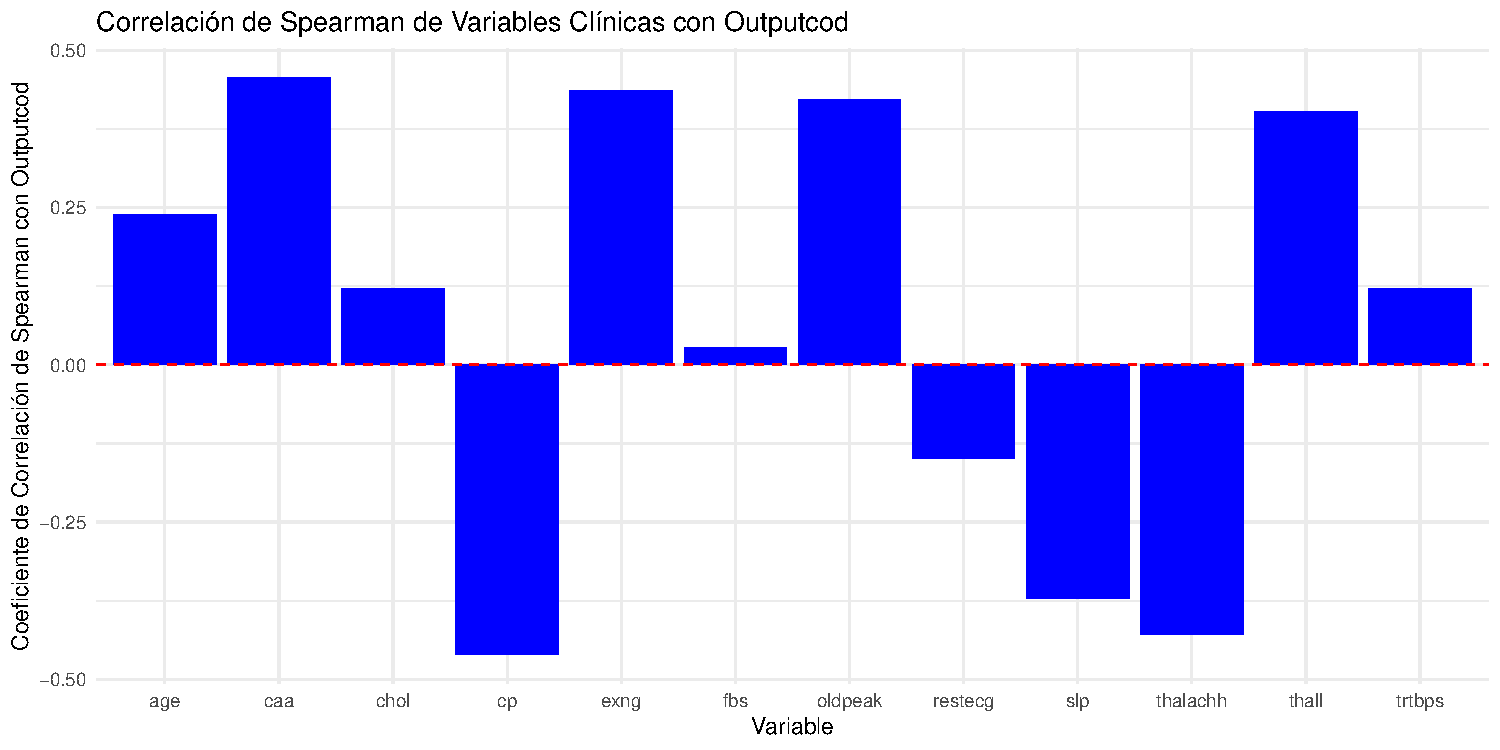
\includegraphics{coyolaf_ChristianOyola-PRA2_files/figure-latex/unnamed-chunk-22-1.pdf}

\begin{itemize}
\item
  Las variables \textbf{caa (número de vasos principales coloreados por
  fluoroscopia)}, \textbf{exng (angina inducida por el ejercicio)},
  \textbf{oldpeak (depresión del ST inducida por el ejercicio en
  relación con el reposo)}, y \textbf{thall (defectos identificados en
  la prueba de talio)} muestran correlaciones positivas con output Esto
  indica que hay una asociación en la que valores más altos de estas
  variables tienden a ir acompañados de un valor más alto en output. Se
  puede indicar de manera preliminar que estas variables pueden
  considerarse factores de riesgo o indicadores de mayor probabilidad de
  dicho evento.
\item
  Por otro lado, \textbf{cp (tipo de dolor en el pecho)}, \textbf{slp
  (la pendiente del segmento ST del ejercicio máximo)} y
  \textbf{thalachh (máxima frecuencia cardíaca alcanzada)}, muestran
  correlaciones negativas con output. Esto significa que valores más
  altos en estas variables están asociados con valores más bajos en
  output, lo cual podría interpretarse como un indicador de menor
  riesgo.
\item
  Las variables \textbf{chol (colesterol sérico)}, \textbf{fbs (azúcar
  en la sangre en ayunas)}, \textbf{restecg (resultados
  electrocardiográficos en reposo)} y \textbf{trtbps (presión arterial
  en reposo)}, presentan correlaciones muy débiles con output, ya sean
  positivas o negativas. Estas débiles correlaciones sugieren que no hay
  una fuerte relación lineal entre estas variables y la variable de
  salida (output).
\end{itemize}

\begin{Shaded}
\begin{Highlighting}[]
\NormalTok{n }\OtherTok{=} \FunctionTok{c}\NormalTok{(}\StringTok{"outputcod"}\NormalTok{, }\StringTok{"age"}\NormalTok{, }\StringTok{"cp"}\NormalTok{, }\StringTok{"trtbps"}\NormalTok{, }\StringTok{"chol"}\NormalTok{, }\StringTok{"fbs"}\NormalTok{, }\StringTok{"restecg"}\NormalTok{, }\StringTok{"thalachh"}\NormalTok{, }\StringTok{"exng"}\NormalTok{, }\StringTok{"oldpeak"}\NormalTok{, }\StringTok{"slp"}\NormalTok{, }\StringTok{"caa"}\NormalTok{, }\StringTok{"thall"}\NormalTok{)}
\NormalTok{factores}\OtherTok{=}\NormalTok{ data\_heart }\SpecialCharTok{\%\textgreater{}\%} \FunctionTok{select}\NormalTok{(}\FunctionTok{all\_of}\NormalTok{(n))}
\NormalTok{res}\OtherTok{\textless{}{-}}\FunctionTok{cor}\NormalTok{(factores)}
\FunctionTok{corrplot}\NormalTok{(res,}\AttributeTok{method=}\StringTok{"color"}\NormalTok{,}\AttributeTok{tl.col=}\StringTok{"black"}\NormalTok{, }\AttributeTok{tl.srt=}\DecValTok{30}\NormalTok{, }\AttributeTok{order =} \StringTok{"AOE"}\NormalTok{,}
\AttributeTok{number.cex=}\FloatTok{0.75}\NormalTok{,}\AttributeTok{sig.level =} \FloatTok{0.01}\NormalTok{, }\AttributeTok{addCoef.col =} \StringTok{"black"}\NormalTok{)}
\end{Highlighting}
\end{Shaded}

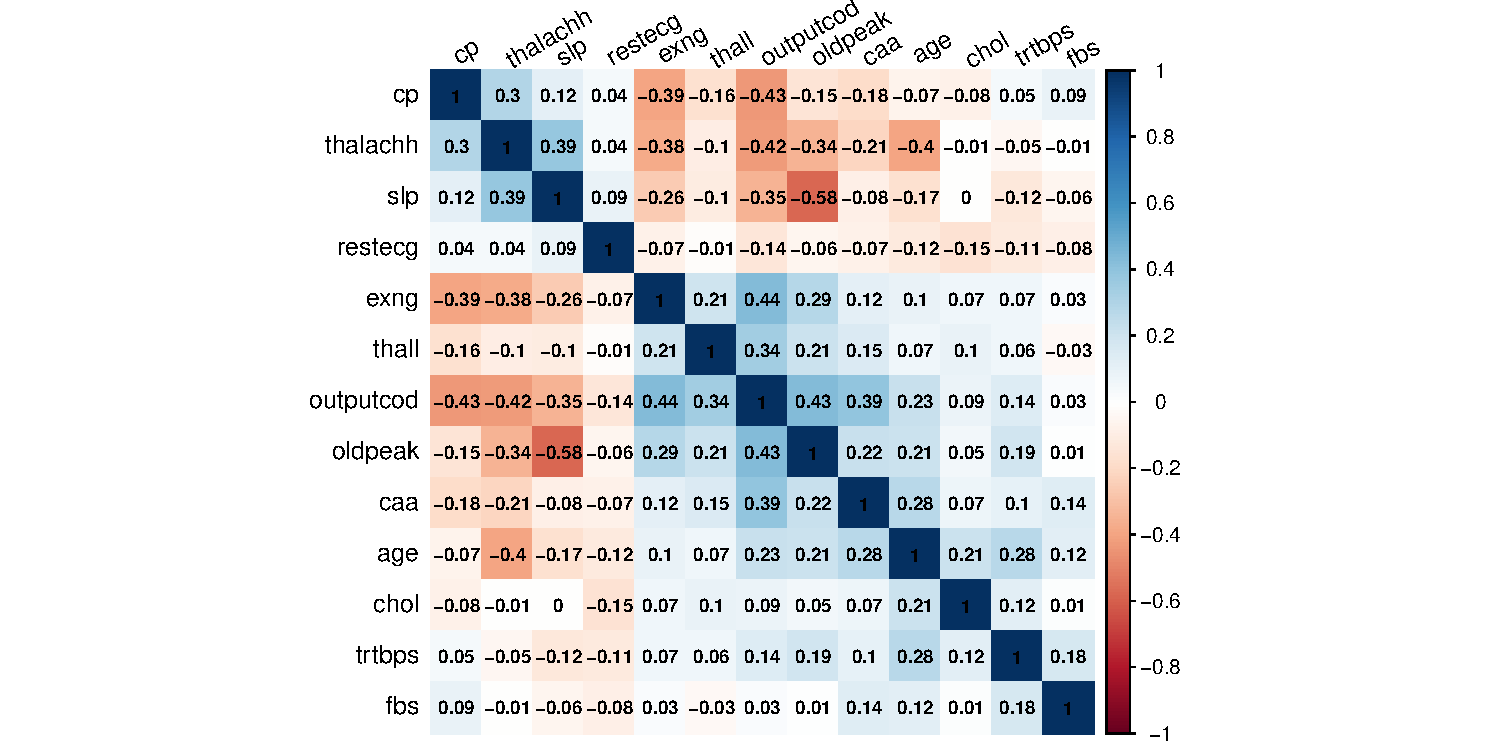
\includegraphics{coyolaf_ChristianOyola-PRA2_files/figure-latex/unnamed-chunk-23-1.pdf}

\hypertarget{construcciuxf3n-del-conjunto-de-datos-final}{%
\section{3 Construcción del conjunto de datos
final}\label{construcciuxf3n-del-conjunto-de-datos-final}}

\hypertarget{recodificaciuxf3n-de-variables}{%
\subsection{3.1 Recodificación de
variables}\label{recodificaciuxf3n-de-variables}}

Se aplica la codificación one-hot en la variable OUTPUT para optimizar
su interpretación por los algoritmos de aprendizaje automático. Este
enfoque garantiza que las categorías se manejen de manera equitativa,
sin asumir jerarquías o secuencias entre ellas.

\begin{Shaded}
\begin{Highlighting}[]
\CommentTok{\# Codificación one{-}hot de la variable "OUTPUT"}
\NormalTok{data\_heart }\OtherTok{\textless{}{-}} \FunctionTok{cbind}\NormalTok{(data\_heart, }\FunctionTok{model.matrix}\NormalTok{(}\SpecialCharTok{\textasciitilde{}}\NormalTok{ output }\SpecialCharTok{{-}} \DecValTok{1}\NormalTok{, data\_heart))}
\FunctionTok{head}\NormalTok{(data\_heart,}\DecValTok{4}\NormalTok{)}
\end{Highlighting}
\end{Shaded}

\begin{verbatim}
##   age       sex cp trtbps chol fbs restecg thalachh exng oldpeak slp caa thall
## 1  63 Masculino  3    145  233   1       0      150    0     2.3   0   0     1
## 2  37 Masculino  2    130  250   0       1      187    0     3.5   0   0     2
## 3  41  Femenino  1    130  204   0       0      172    0     1.4   2   0     2
## 4  56 Masculino  1    120  236   0       1      178    0     0.8   2   0     2
##         output outputcod outputheart-attack outputno-heart-attack
## 1 heart-attack         1                  1                     0
## 2 heart-attack         1                  1                     0
## 3 heart-attack         1                  1                     0
## 4 heart-attack         1                  1                     0
\end{verbatim}

\hypertarget{discretizaciuxf3n-y-codificaciuxf3n-de-la-variable-age}{%
\subsection{3.2 Discretización y codificación de la variable
AGE}\label{discretizaciuxf3n-y-codificaciuxf3n-de-la-variable-age}}

Procederemos a discretizar la variable AGE definiendo grupos como
``jóvenes'' (menores de 30 años), ``Mediana\_edad'' (30-50 años), y
``Mayores'' (mayores de 50 años):

\begin{Shaded}
\begin{Highlighting}[]
\CommentTok{\# Discretización basada en criterios de dominio}
\NormalTok{data\_heart}\SpecialCharTok{$}\NormalTok{age\_group }\OtherTok{\textless{}{-}} \FunctionTok{cut}\NormalTok{(data\_heart}\SpecialCharTok{$}\NormalTok{age, }\AttributeTok{breaks =} \FunctionTok{c}\NormalTok{(}\DecValTok{0}\NormalTok{, }\DecValTok{30}\NormalTok{, }\DecValTok{50}\NormalTok{, }\ConstantTok{Inf}\NormalTok{),}
                       \AttributeTok{labels =} \FunctionTok{c}\NormalTok{(}\StringTok{"Jóven"}\NormalTok{, }\StringTok{"Mediana\_edad"}\NormalTok{, }\StringTok{"Mayor\_edad"}\NormalTok{))}
\FunctionTok{head}\NormalTok{(data\_heart,}\DecValTok{4}\NormalTok{)}
\end{Highlighting}
\end{Shaded}

\begin{verbatim}
##   age       sex cp trtbps chol fbs restecg thalachh exng oldpeak slp caa thall
## 1  63 Masculino  3    145  233   1       0      150    0     2.3   0   0     1
## 2  37 Masculino  2    130  250   0       1      187    0     3.5   0   0     2
## 3  41  Femenino  1    130  204   0       0      172    0     1.4   2   0     2
## 4  56 Masculino  1    120  236   0       1      178    0     0.8   2   0     2
##         output outputcod outputheart-attack outputno-heart-attack    age_group
## 1 heart-attack         1                  1                     0   Mayor_edad
## 2 heart-attack         1                  1                     0 Mediana_edad
## 3 heart-attack         1                  1                     0 Mediana_edad
## 4 heart-attack         1                  1                     0   Mayor_edad
\end{verbatim}

\begin{Shaded}
\begin{Highlighting}[]
\CommentTok{\# Codificación one{-}hot de la variable "AGE\_Group"}
\NormalTok{data\_heart }\OtherTok{\textless{}{-}} \FunctionTok{cbind}\NormalTok{(data\_heart, }\FunctionTok{model.matrix}\NormalTok{(}\SpecialCharTok{\textasciitilde{}}\NormalTok{ age\_group }\SpecialCharTok{{-}} \DecValTok{1}\NormalTok{, data\_heart))}
\CommentTok{\# Verificar la codificación one{-}hot}
\FunctionTok{head}\NormalTok{(data\_heart,}\DecValTok{4}\NormalTok{)}
\end{Highlighting}
\end{Shaded}

\begin{verbatim}
##   age       sex cp trtbps chol fbs restecg thalachh exng oldpeak slp caa thall
## 1  63 Masculino  3    145  233   1       0      150    0     2.3   0   0     1
## 2  37 Masculino  2    130  250   0       1      187    0     3.5   0   0     2
## 3  41  Femenino  1    130  204   0       0      172    0     1.4   2   0     2
## 4  56 Masculino  1    120  236   0       1      178    0     0.8   2   0     2
##         output outputcod outputheart-attack outputno-heart-attack    age_group
## 1 heart-attack         1                  1                     0   Mayor_edad
## 2 heart-attack         1                  1                     0 Mediana_edad
## 3 heart-attack         1                  1                     0 Mediana_edad
## 4 heart-attack         1                  1                     0   Mayor_edad
##   age_groupJóven age_groupMediana_edad age_groupMayor_edad
## 1              0                     0                   1
## 2              0                     1                   0
## 3              0                     1                   0
## 4              0                     0                   1
\end{verbatim}

\hypertarget{aplicaciuxf3n-de-pruebas-estadisticas}{%
\section{4 Aplicación de pruebas
estadisticas}\label{aplicaciuxf3n-de-pruebas-estadisticas}}

\hypertarget{regresiuxf3n-loguxedstica}{%
\subsection{4.1 Regresión logística}\label{regresiuxf3n-loguxedstica}}

\begin{Shaded}
\begin{Highlighting}[]
\CommentTok{\# Establecer una semilla para reproducibilidad}
\FunctionTok{set.seed}\NormalTok{(}\DecValTok{123}\NormalTok{)}
\CommentTok{\# Dividir los datos en conjuntos de entrenamiento y prueba}
\NormalTok{split }\OtherTok{\textless{}{-}} \FunctionTok{sample.split}\NormalTok{(data\_heart}\SpecialCharTok{$}\NormalTok{trtbps, }\AttributeTok{SplitRatio =} \FloatTok{0.7}\NormalTok{)}
\NormalTok{train\_data }\OtherTok{\textless{}{-}} \FunctionTok{subset}\NormalTok{(data\_heart, split }\SpecialCharTok{==} \ConstantTok{TRUE}\NormalTok{)}
\NormalTok{test\_data }\OtherTok{\textless{}{-}} \FunctionTok{subset}\NormalTok{(data\_heart, split }\SpecialCharTok{==} \ConstantTok{FALSE}\NormalTok{)}
\CommentTok{\# Ajustar el modelo de regresión logistica con los datos de entrenamiento}
\NormalTok{ModlgF }\OtherTok{\textless{}{-}} \FunctionTok{glm}\NormalTok{(output }\SpecialCharTok{\textasciitilde{}}\NormalTok{ age }\SpecialCharTok{+}\NormalTok{ sex }\SpecialCharTok{+}\NormalTok{ trtbps }\SpecialCharTok{+}\NormalTok{ chol }\SpecialCharTok{+}\NormalTok{ fbs }\SpecialCharTok{+}\NormalTok{ exng }\SpecialCharTok{+}\NormalTok{ oldpeak }\SpecialCharTok{+}\NormalTok{ caa }\SpecialCharTok{+}\NormalTok{ thall }\SpecialCharTok{+}\NormalTok{cp }\SpecialCharTok{+}\NormalTok{ trtbps }\SpecialCharTok{+}\NormalTok{ restecg }\SpecialCharTok{+}\NormalTok{ slp }\SpecialCharTok{+}\NormalTok{ thalachh, }
                        \AttributeTok{data =}\NormalTok{ train\_data, }\AttributeTok{family =} \FunctionTok{binomial}\NormalTok{())}
\FunctionTok{summary}\NormalTok{(ModlgF)}
\end{Highlighting}
\end{Shaded}

\begin{verbatim}
## 
## Call:
## glm(formula = output ~ age + sex + trtbps + chol + fbs + exng + 
##     oldpeak + caa + thall + cp + trtbps + restecg + slp + thalachh, 
##     family = binomial(), data = train_data)
## 
## Coefficients:
##               Estimate Std. Error z value Pr(>|z|)    
## (Intercept)  -1.986500   3.161683  -0.628 0.529804    
## age          -0.006412   0.029600  -0.217 0.828518    
## sexMasculino  1.822565   0.580850   3.138 0.001702 ** 
## trtbps        0.017612   0.011666   1.510 0.131113    
## chol          0.004454   0.004432   1.005 0.314962    
## fbs           0.239072   0.602680   0.397 0.691602    
## exng          0.911284   0.501707   1.816 0.069314 .  
## oldpeak       0.422185   0.234587   1.800 0.071909 .  
## caa           0.944318   0.246665   3.828 0.000129 ***
## thall         0.994650   0.337759   2.945 0.003231 ** 
## cp           -0.818427   0.220288  -3.715 0.000203 ***
## restecg      -0.230784   0.406824  -0.567 0.570523    
## slp          -0.501202   0.404063  -1.240 0.214825    
## thalachh     -0.029569   0.012650  -2.338 0.019412 *  
## ---
## Signif. codes:  0 '***' 0.001 '**' 0.01 '*' 0.05 '.' 0.1 ' ' 1
## 
## (Dispersion parameter for binomial family taken to be 1)
## 
##     Null deviance: 296.37  on 214  degrees of freedom
## Residual deviance: 156.58  on 201  degrees of freedom
## AIC: 184.58
## 
## Number of Fisher Scoring iterations: 6
\end{verbatim}

\begin{Shaded}
\begin{Highlighting}[]
\FunctionTok{set.seed}\NormalTok{(}\DecValTok{123}\NormalTok{)}
\NormalTok{split }\OtherTok{\textless{}{-}} \FunctionTok{sample.split}\NormalTok{(data\_heart}\SpecialCharTok{$}\NormalTok{trtbps, }\AttributeTok{SplitRatio =} \FloatTok{0.7}\NormalTok{)}
\CommentTok{\# Ajustar el modelo de regresión logistica con los datos de entrenamiento}
\NormalTok{ModlgF }\OtherTok{\textless{}{-}} \FunctionTok{glm}\NormalTok{(output }\SpecialCharTok{\textasciitilde{}}\NormalTok{ age }\SpecialCharTok{+}\NormalTok{ sex }\SpecialCharTok{+}\NormalTok{ exng }\SpecialCharTok{+}\NormalTok{ oldpeak }\SpecialCharTok{+}\NormalTok{ caa }\SpecialCharTok{+}\NormalTok{ thall }\SpecialCharTok{+}\NormalTok{cp }\SpecialCharTok{+}\NormalTok{ slp }\SpecialCharTok{+}\NormalTok{ thalachh, }
                        \AttributeTok{data =}\NormalTok{ train\_data, }\AttributeTok{family =} \FunctionTok{binomial}\NormalTok{())}
\FunctionTok{summary}\NormalTok{(ModlgF)}
\end{Highlighting}
\end{Shaded}

\begin{verbatim}
## 
## Call:
## glm(formula = output ~ age + sex + exng + oldpeak + caa + thall + 
##     cp + slp + thalachh, family = binomial(), data = train_data)
## 
## Coefficients:
##              Estimate Std. Error z value Pr(>|z|)    
## (Intercept)  -0.81088    2.89925  -0.280 0.779717    
## age           0.01490    0.02673   0.557 0.577211    
## sexMasculino  1.55337    0.50692   3.064 0.002182 ** 
## exng          0.88628    0.48856   1.814 0.069669 .  
## oldpeak       0.46042    0.22596   2.038 0.041586 *  
## caa           0.88740    0.23863   3.719 0.000200 ***
## thall         1.03036    0.32506   3.170 0.001525 ** 
## cp           -0.75470    0.20684  -3.649 0.000264 ***
## slp          -0.49841    0.39594  -1.259 0.208102    
## thalachh     -0.02282    0.01147  -1.989 0.046735 *  
## ---
## Signif. codes:  0 '***' 0.001 '**' 0.01 '*' 0.05 '.' 0.1 ' ' 1
## 
## (Dispersion parameter for binomial family taken to be 1)
## 
##     Null deviance: 296.37  on 214  degrees of freedom
## Residual deviance: 160.55  on 205  degrees of freedom
## AIC: 180.55
## 
## Number of Fisher Scoring iterations: 6
\end{verbatim}

Según el modelo con las variables con correlación que muestran una
fuerte relación con la variable dependiente ``output'', y que se pueden
considerar estadisticamente significativas son: \textbf{sexMasculino},
\textbf{exng}, \textbf{oldpeak}, \textbf{caa}, \textbf{thall},
\textbf{cp}, \textbf{thalachh} lo que puede sugerir que estos factores
son relevantes en la predicción de `output'.

\hypertarget{matruxedz-de-confusiuxf3n}{%
\subsection{4.2 Matríz de confusión}\label{matruxedz-de-confusiuxf3n}}

\begin{Shaded}
\begin{Highlighting}[]
\CommentTok{\# probabilidades predichas por el modelo}
\NormalTok{probabilidades }\OtherTok{\textless{}{-}} \FunctionTok{predict}\NormalTok{(ModlgF, }\AttributeTok{newdata =}\NormalTok{ test\_data, }\AttributeTok{type =} \StringTok{"response"}\NormalTok{)}
\CommentTok{\# conversión de las probabilidades en predicciones binarias usando el umbral de 0.7}
\NormalTok{predicciones }\OtherTok{\textless{}{-}} \FunctionTok{ifelse}\NormalTok{(probabilidades }\SpecialCharTok{\textgreater{}=} \FloatTok{0.7}\NormalTok{, }\DecValTok{1}\NormalTok{, }\DecValTok{0}\NormalTok{)}
\CommentTok{\# matriz de confusión frente a valores reales}
\NormalTok{matriz\_confusion }\OtherTok{\textless{}{-}} \FunctionTok{table}\NormalTok{(}\AttributeTok{predic =}\NormalTok{ predicciones, }\AttributeTok{val =}\NormalTok{ test\_data}\SpecialCharTok{$}\NormalTok{output)}
\CommentTok{\# sensibilidad y especificidad}
\NormalTok{sensibilidad }\OtherTok{\textless{}{-}}\NormalTok{ matriz\_confusion[}\DecValTok{2}\NormalTok{, }\DecValTok{2}\NormalTok{] }\SpecialCharTok{/} \FunctionTok{sum}\NormalTok{(matriz\_confusion[}\DecValTok{2}\NormalTok{, ])}
\NormalTok{especificidad }\OtherTok{\textless{}{-}}\NormalTok{ matriz\_confusion[}\DecValTok{1}\NormalTok{, }\DecValTok{1}\NormalTok{] }\SpecialCharTok{/} \FunctionTok{sum}\NormalTok{(matriz\_confusion[}\DecValTok{1}\NormalTok{, ])}
\FunctionTok{print}\NormalTok{(matriz\_confusion)}
\end{Highlighting}
\end{Shaded}

\begin{verbatim}
##       val
## predic heart-attack no-heart-attack
##      0           45               8
##      1            3              32
\end{verbatim}

\textbf{Verdaderos Negativos:} 45 casos donde el modelo predijo
correctamente que no ocurriría un ataque cardíaco (no-heart-attack) y
efectivamente no ocurrió.

\textbf{Falsos Positivos:} 8 casos donde el modelo predijo
incorrectamente que ocurriría un ataque cardíaco (heart-attack), pero en
realidad no sucedió.

\textbf{Falsos Negativos:} 3 casos dobde el modelo falló al predecir un
ataque cardíaco; es decir, predijo que no habría ataque cardíaco
(no-heart-attack), pero realmente sí ocurrió.

\textbf{Verdaderos Positivos:} 32 casos donde el modelo predijo
correctamente la ocurrencia de un ataque cardíaco (heart-attack) y este
realmente sucedió.

\begin{Shaded}
\begin{Highlighting}[]
\FunctionTok{print}\NormalTok{(}\FunctionTok{paste}\NormalTok{(}\StringTok{"Sensibilidad:"}\NormalTok{, sensibilidad))}
\end{Highlighting}
\end{Shaded}

\begin{verbatim}
## [1] "Sensibilidad: 0.914285714285714"
\end{verbatim}

\begin{Shaded}
\begin{Highlighting}[]
\FunctionTok{print}\NormalTok{(}\FunctionTok{paste}\NormalTok{(}\StringTok{"Especificidad:"}\NormalTok{, especificidad))}
\end{Highlighting}
\end{Shaded}

\begin{verbatim}
## [1] "Especificidad: 0.849056603773585"
\end{verbatim}

El modelo predice de manera satisfactoria los casos en los cuales se
presenta un ataque cardiaco relacionado con las variables identificadas
que pueden poternciar esta problemática, así mismo, el modelo responde a
identificar de manera relativamente óptima, los casos en los que no se
presenta este escenario.

\hypertarget{conclusiones}{%
\section{5 Conclusiones}\label{conclusiones}}

\textbf{Principales Factores Predictivos de un Ataque Cardíaco:}

Los factores que mostraron una asociación estadísticamente significativa
con la variable dependiente output incluyen sexMasculino, cp, thalachh,
caa y thall.

\begin{itemize}
\tightlist
\item
  \emph{sexMasculino:} Ser hombre se asoció con un aumento en las odds
  de output.
\item
  \emph{cp:} Una disminución en esta variable (tipo de dolor en el
  pecho) se asoció con un aumento en las odds de output, lo que sugiere
  que la mayoría de escenarios en los que se da un ataque cardiaco el
  paciente es asintomático, o presenta un dolor torácico relacionado con
  una angina típica.
\item
  \emph{thalachh:} Una disminución en la máxima frecuencia cardíaca
  alcanzada se asoció con un aumento en las odds de output. Cabe indicar
  que esta variable está relacionada con la actividad física, lo que
  puede sugerir que los individuos que realizan un esfuerzo físico
  presentan esta patología.
\item
  \emph{caa:} Aunque en la gráfica de densidad observamos un pico rojo
  en caa = 0, el modelo de regresión logística reveló que un mayor
  número de caa se asocia con un aumento significativo en las odds de
  output. Esto puede indicar que, si bien tener caa = 0 es común entre
  los pacientes que han tenido un ataque cardíaco, tener un número mayor
  de vasos coloreados está aún más fuertemente asociado con el riesgo de
  ataque cardíaco.
\item
  \emph{thall:} Un aumento en esta variable se asoció con un aumento en
  las odds de output.
\end{itemize}

\textbf{Efecto del Ejercicio y la Dieta en el Riesgo de Ataques
Cardíacos:}

El ejercicio, representado por variables como thalachh (máxima
frecuencia cardíaca alcanzada) y exng (angina inducida por el
ejercicio), mostró que una menor frecuencia cardíaca máxima y la
presencia de angina están asociadas con un mayor riesgo, aunque la
significancia de exng es marginal. La dieta, que podría influir en
variables como chol (colesterol sérico) y fbs (azúcar en la sangre en
ayunas), no mostró una relación estadísticamente significativa con el
riesgo de ataque cardíaco en este modelo.

\textbf{Diferencias en Síntomas y Factores de Riesgo entre Hombres y
Mujeres:}

La variable sexMasculino mostró que ser hombre está asociado con un
mayor riesgo de ataque cardíaco en este modelo. Esto sugiere que puede
haber diferencias en los factores de riesgo y posiblemente en los
síntomas entre hombres y mujeres.

\textbf{Cambio en el Riesgo y Presentación de Enfermedades Cardíacas con
la Edad:}

La variable age no mostró una asociación significativa con output en
este modelo, lo que sugiere que, dentro del rango de edad del conjunto
de datos, la edad por sí sola no es un predictor significativo. Sin
embargo, esto no significa que la edad no sea un factor en el riesgo
general de enfermedades cardíacas.

\end{document}
